        %%******************************************%%
        %%                                          %%
        %%        Modello di tesi di laurea         %%
        %%            di Andrea Giraldin            %%
        %%                                          %%
        %%             2 novembre 2012              %%
        %%                                          %%
        %%******************************************%%

\begin{document}
    \frontmatter
    \begin{titlepage}
    \begin{center}
        \begin{LARGE}
            \textbf{\myUni}\\
        \end{LARGE}

        \vspace{10pt}

        \begin{Large}
            \textsc{\myDepartment}\\
        \end{Large}

        \vspace{10pt}

        \begin{large}
            \textsc{\myFaculty}\\
        \end{large}

        \vspace{30pt}
        \begin{figure}[htbp]
            \centering
            
\includegraphics[height=6cm]{unipd-logo}
        \end{figure}
        \vspace{30pt}

        \begin{LARGE}
            \textbf{\myTitle}\\
        \end{LARGE}

        \vspace{10pt}

        \begin{large}
            \textsl{\myDegree}\\
        \end{large}

        \vspace{40pt}

        \begin{large}
            \begin{flushleft}
                \textit{Relatore}\\
                \vspace{5pt}
                \profTitle\ \myProf
            \end{flushleft}

            % You can tweak the spacing to have professor and student names on the same line
            % useful if the page is broken by a long thesis title and you need more space
            %\vspace{-52pt}

            \begin{flushright}
                \textit{Laureando}\\
                \vspace{5pt}
                \myName \\
                %\vspace{5pt}
                %\textit{Matricola} \myID
            \end{flushright}
        \end{large}

        \vspace{40pt}

        \line(1, 0){338} \\
        \begin{normalsize}
            \textsc{Anno Accademico \myAA}
        \end{normalsize}
    \end{center}
\end{titlepage}

    \clearpage
\phantomsection
\thispagestyle{empty}

\hfill
\vfill

\noindent\myName: \textit{\myTitle,}
\myDegree,
\textcopyright\ \myTime.

    \cleardoublepage
\phantomsection
\pdfbookmark{Sommario}{Sommario}
\begingroup
\let\clearpage\relax
\let\cleardoublepage\relax
\let\cleardoublepage\relax

\chapter*{Sommario}

Il presente documento esibisce un resoconto dell'attività di stage condotta dalla laureanda \myName \space presso 
l'azienda Zucchetti S.p.A. (sede di Padova) per una durata di circa trecento ore.\\

\noindent Esso si propone di esaminare il campo della \emph{data visualization} e delle infografiche, riportandone 
anche un'applicazione pratica effettuata tramite la libreria D3.js. 
%L'obiettivo dello stage era, infatti, sviluppare un sistema di visualizzazione innovativo e interattivo 
%per i risultati ottenuti da algoritmi basati su Intelligenza Artificiale.
\\

\noindent Nello specifico, il documento è strutturato come segue. \\
La parte introduttiva delinea le aspettative iniziali e i piani per lo stage, 
inquadrando il tutto nel contesto aziendale. \\
Successivamente, vengono esplorati i fondamenti della \emph{data visualization} e analizzate le caratteristiche 
delle infografiche. Inoltre, una particolare attenzione viene rivolta anche all'individuazione di meccanismi 
che ottimizzino la scelta di tali raffigurazioni.\\
In seguito, si approfondisce, attraverso un caso pratico, la creazione di infografiche interattive 
realizzate mediante la libreria D3.js.\\
Infine, il documento si conclude con una riflessione sull'esperienza effettuata, inclusi i risultati ottenuti 
e le considerazioni personali sul percorso compiuto.\\

\noindent Per quanto riguarda il documento in sé, si riportano di seguito le convenzioni tipografiche adottate:
\begin{itemize}
    \item gli acronimi, le abbreviazioni e i termini ambigui o di uso non comune menzionati vengono definiti nel glossario, situato alla fine del presente documento;
    \item per la prima occorrenza dei termini riportati nel glossario viene utilizzata la seguente nomenclatura: \emph{parola}\glsfirstoccur;
    \item i termini in lingua straniera o facenti parti del gergo tecnico sono evidenziati con il carattere \emph{corsivo}.
\end{itemize}


%\vfill

%\selectlanguage{english}
%\pdfbookmark{Abstract}{Abstract}
%\chapter*{Abstract}

%\selectlanguage{italian}

\endgroup

\vfill

    \cleardoublepage
\phantomsection
\pdfbookmark{Ringraziamenti}{ringraziamenti}

\begin{flushright}{
    \slshape
    ``I was born to be anything I wanted to be''} \\
    \medskip
    --- Palaye Royale, ``Anxiety''
\end{flushright}


\bigskip

\begingroup
\let\clearpage\relax
\let\cleardoublepage\relax
\let\cleardoublepage\relax

\chapter*{Ringraziamenti}

\noindent \textit{In primo luogo, vorrei ringraziare il Prof. \myProf, relatore della mia tesi, per l'aiuto fornitomi durante la stesura del lavoro.}\\

\noindent \textit{In secondo luogo, desidero ringraziare i miei genitori per avermi dato l'opportunità di raggiungere questo traguardo.}\\

\noindent \textit{Infine, un grazie speciale va anche ai miei amici per le risate e i momenti condivisi insieme durante questi anni e al mio ragazzo, Filippo, per avermi supportato e sopportato anche nei momenti più difficili.}\\

\bigskip

% da riscrivere sta cosa ew

\noindent\textit{\myLocation, \myTime}
\hfill \myName

\endgroup

    \cleardoublepage
\pdfbookmark{\contentsname}{tableofcontents}
\setcounter{tocdepth}{2}
\tableofcontents
%\markboth{\contentsname}{\contentsname}
\clearpage

\begingroup
    \let\clearpage\relax
    \let\cleardoublepage\relax
    \let\cleardoublepage\relax

    % Figures list
    \phantomsection
    \pdfbookmark{\listfigurename}{lof}
    \listoffigures

    \vspace*{8ex}

    % Tables list
    \phantomsection
    \pdfbookmark{\listtablename}{lot}
    \listoftables

    \vspace*{8ex}
\endgroup

\cleardoublepage

    \cleardoublepage

    \mainmatter
    \chapter{Introduzione}
\label{cap:introduzione}
\intro{In questo capitolo verranno delineate le aspettative iniziali e i piani per lo stage, 
inquadrando il tutto nel contesto aziendale.}

\section{Il contesto di riferimento}
\subsection{L'azienda ospitante}
Zucchetti S.p.A. nasce nel 1978 da un'intuizione di Domenico ``Mino'' Zucchetti, 
che per primo in Italia realizzò un software capace di realizzare la dichiarazione
dei redditi in maniera automatizzata.
Questo prodotto ebbe un grande successo e l'azienda iniziò quindi a produrre
software per automatizzare altre procedure contabili aziendali.

\begin{figure}[h!] 
    \centering 
    
\includegraphics[width=0.6\columnwidth]{zucchetti-logo.png} 
    \caption{Logo Zucchetti S.p.A.}
\end{figure}

\noindent A oggi, Zucchetti è una delle principali aziende in Italia nel settore ICT 
(\emph{Information and Communication Technology}) e un attore sempre 
più rilevante sul mercato internazionale.
Il gruppo può infatti contare più di 9.000 dipendenti distribuiti in 15 paesi 
e oltre 700.000 clienti presenti in più di 50 nazioni.

Oltre al consolidamento della sua presenza sul territorio, Zucchetti ha anche 
ampliato la sua offerta di prodotti.
Essa fornisce gestionali aziendali e soluzioni ERP (\emph{Enterprise Resource Planning})
per la gestione del personale, le comunicazione aziendali, la rilevazione delle 
presenze e degli accessi, etc.. 
Zucchetti opera, inoltre, nel campo dell'e-business e della business intelligence e
offre servizi per robotica, automazione, sicurezza informatica e server farm.

\subsubsection{Servizi offerti}
La \emph{mission} di Zucchetti è quella di supportare le aziende nel migliorare
la loro competitività ed efficienza operativa attraverso soluzioni innovative e 
di qualità.
A tal fine, Zucchetti S.p.A. fornisce ai suoi clienti:
\begin{itemize}
    \item \textbf{Un supporto pre-vendita}, analizzando e studiando le soluzioni 
    che meglio si adattano al problema;
    \item \textbf{Un supporto post-vendita}, installando il prodotto e 
    offrendo supporto tecnico;
    \item \textbf{Una formazione del personale}, per consentire al cliente di 
    sfruttare al meglio il prodotto acquistato;
    \item \textbf{Un aggiornamento costante}, per restare al passo con le nuove
    tecnologie e le nuove normative in materia fiscale, contabile e amministrativa.
\end{itemize} 

\subsubsection{Clientela target}
Zucchetti S.p.A. si rivolge a una vasta gamma di clientela, comprendente imprese
di ogni dimensione e settore, ma anche professionisti e associazioni di categoria, 
oltre che CAF e Pubblica Amministrazione. 
La sua offerta diversificata di soluzioni software e servizi tecnologici è pensata 
infatti per soddisfare le esigenze specifiche di ciascun segmento di mercato.


\section{Aspettative iniziali}
\subsection{La proposta di stage}
Lo scopo del progetto di stage è quello di sviluppare un sistema di visualizzazione interattiva dei dati che 
fornisca agli utenti una comprensione non convenzionale, ma pur sempre intuitiva, delle analisi effettuate. 
Per realizzare tale visualizzazione viene proposto l'utilizzo della libreria JavaScript ``D3.js'', nota per la 
sua flessibilità e capacità di creare visualizzazioni grafiche dinamiche e coinvolgenti.

A tal fine, è necessario studiare e analizzare in profondità le varie modalità di rappresentazione
grafica dei dati, focalizzandosi sull'identificazione delle tecniche più idonee per rendere chiari e
informativi i vari tipi di dati possibili. A partire da questo studio, si potrà passare alla creazione di un'infografica
web, che combinerà grafici realizzati tramite ``D3.js'' con altri elementi aggiuntivi di chiarimento. Una
volta completata l'infografica, si prevede di sviluppare un template riutilizzabile per future rappresentazioni
simili e verificarne l'efficacia e l'utilità mediante adeguati metodi di valutazione. 

Questo progetto di stage offre dunque l'opportunità di approfondire la propria conoscenza dei seguenti campi:
\begin{itemize}
    \item \textbf{Data visualization}, attraverso lo studio di infografiche e, in particolare, di grafici informativi;
    \item \textbf{Utilizzo della libreria D3.js}, attraverso la creazione di grafici dinamici e interattivi inseriti all'interno dell'infografica;
    \item \textbf{Sviluppo Web con HTML/CSS/JS}, attraverso la realizzazione di un'interfaccia web che implementi l'infografica.
\end{itemize}

\subsection{Pianificazione delle attività}
Si riporta di seguito la pianificazione delle attività di stage suddivise 
nelle otto settimane di lavoro previste.

\begin{itemize}
    \item \textbf{Prima Settimana - Formazione}
    \begin{itemize}
        \item Introduzione e approfondimento sui principi chiave e sulle metodologie della \textit{Data Visualization};
        \item Formazione sulle tecnologie da adottare, in particolare sulla libreria ``D3.js''.
    \end{itemize}
    \item \textbf{Seconda Settimana - Selezione e sviluppo di grafici} 
    \begin{itemize}
        \item Identificazione dei criteri per la scelta del tipo di grafico più adatto, considerando la struttura dei dati e gli obiettivi della visualizzazione;
        \item Sviluppo dei grafici individuati utilizzando la libreria ``D3.js''.
    \end{itemize}
    \item \textbf{Terza Settimana - Integrazione di algoritmi a grafici} 
    \begin{itemize}
        \item Sviluppo di grafici avanzati, che integrano algoritmi, attraverso l'uso di ``D3.js''.
    \end{itemize}
    \item \textbf{Quarta Settimana - Test e Documentazione} 
    \begin{itemize}
        \item Realizzazione di test che verifichino la bontà del codice prodotto nelle settimane precedenti;
        \item Produzione di documentazione riguardante il prodotto realizzato.
    \end{itemize}
    \item \textbf{Quinta Settimana - Approfondimento sulle infografiche} 
    \begin{itemize}
        \item Ricerca approfondita di informazioni e guide riguardanti il concetto di infografica;
        \item Raccolta di elementi grafici e di design da accompagnare ai grafici per migliorarne la comprensibilità e l'attrattività visiva;
        \item Realizzazione preliminare dell'infografica utilizzando HTML, CSS e JavaScript.
    \end{itemize}
    \item \textbf{Sesta Settimana - Completamento dell'infografica e crezione del template} 
    \begin{itemize}
        \item Ultimazione dell'infografica in HTML, CSS e JavaScript;
        \item Creazione di un template dell'infografica, riutilizzabile per future analisi simili.
    \end{itemize}
    \item \textbf{Settima Settimana - Metodi di validazione dell'infografica} 
    \begin{itemize}
        \item Individuazione di criteri che permettano di valutare la qualità dell'infografica (e.g. \textit{chatbot} con LLM che interagisce con l'utente sull'infografica ottenendo, indirettamente, il suo feedback per miglioramenti futuri);
        \item Implementazione dei metodi di validazione individuati.
    \end{itemize}
    \item \textbf{Ottava Settimana - Test e Documentazione} 
    \begin{itemize}
        \item Realizzazione di test che verifichino la bontà del codice prodotto nelle settimane precedenti;
        \item Produzione di documentazione riguardante il prodotto realizzato.
    \end{itemize}
\end{itemize}

\subsection{Obiettivi fissati}
Sono fissati i seguenti obiettivi da raggiungere attraverso le attività sopraelencate.

\subsubsection{Obiettivi obbligatori}
\begin{itemize}
    \item \textbf{O01}: Comprendere i principi fondamentali della \textit{Data Visualization};
    \item \textbf{O02}: Selezionare il grafico più adatto per tipo di struttura dati e obiettivo della visualizzazione;
    \item \textbf{O03}: Realizzare grafici informativi e interattivi utilizzando ``D3.js'';
    \item \textbf{O04}: Realizzare un'infografica web funzionante in HTML/CSS/JS che visualizzi i risultati degli algoritmi di intelligenza ertificiale e \textit{machine learning};
    \item \textbf{O05}: Creare un template dell'infografica;
    \item \textbf{O06}: Individuare dei metodi di validazione dell'infografica.
\end{itemize}

\subsubsection{Obiettivi desiderabili}
\begin{itemize}
    \item \textbf{D01}: Sviluppare infografiche alternative;
    \item \textbf{D02}: Implementare un chatbot con LLM che interagisca con l'utente sull'infografica.
\end{itemize}

\subsection{Vincoli}
Si riportano di seguito i vincoli imposti per lo svolgimento dell'attività di stage.

\subsubsection{Vincoli temporali}
La durata dello stage è di otto settimane, per un totale complessivo compreso tra le 300 e le 320 ore in base alla necessità.
Gli orari di lavoro sono dal lunedì al venerdì, dalle ore 9.00 alle ore 18:00, con pausa pranzo dalle 13:00 alle 14:00.

\subsubsection{Vincoli tecnologici}
La proposta di stage prevede l'utilizzo della libreria ``D3.js'' per lo sviluppo
di grafici interattivi. Questi andranno poi a inserirsi in infografiche web da 
sviluppare attraverso HTML, CSS e JavaScript.
Non sono stati imposti limiti ulteriori su eventuali tecnologie aggiuntive.

Per una specifica delle tecnologie effettuate si rimanda alla sezione apposita \ref{subsec:tecnologie}.

% motivazioni personali ?

%analisi preventiva rischi
%Durante la fase di analisi iniziale sono stati individuati alcuni possibili rischi a cui si potrà andare incontro.
%Si è quindi proceduto a elaborare delle possibili soluzioni per far fronte a tali rischi.\\

%\begin{risk}{Performance del simulatore hardware}
 %   \riskdescription{le performance del simulatore hardware e la comunicazione con questo potrebbero risultare lenti o non abbastanza buoni da causare il fallimento dei test}
  %  \risksolution{coinvolgimento del responsabile a capo del progetto relativo il simulatore hardware}
   % \label{risk:hardware-simulator} 
%\end{risk}
    \chapter{Data visualization}
\label{cap:studio_data_viz}
\intro{In questo capitolo verrà presentata una panoramica della \gls{datavizg}, spiegandone caratteristiche, usi e principi.
Viene inoltre proposto un metodo di classificazione dei grafici per ottimizzare le visualizzazioni.}\\

\section{Definizione e applicazioni}
\subsection{La necessità di rappresentare i dati}
%INTRO + CAP 1: “Design della mente – infografica e data viz” di Paolo Bottazini, Michele Gotuzzo
La visualizzazione dei dati ha una tradizione millenaria. Sin dagli albori della civiltà umana, 
le persone hanno sviluppato metodi per rappresentare visivamente i dati al fine di renderli più facili da comprendere, 
memorizzare e trasmettere.
Negli ultimi decenni, tuttavia, questa esigenza ha conosciuto un incremento senza precedenti.

Viviamo infatti nell'epoca dell'\gls{infoloadg} e dei \gls{bigdatag}, dove le informazioni
arrivano con una velocità, un volume e una varietà così travolgenti che non siamo in grado di comprenderli se non attraverso
un ulteriore strato di astrazione.
Tale condizione si deve soprattutto allo sviluppo delle tecnologie digitali, grazie alle quali siamo arrivati a disporre di una quantità 
apparentemente infinita di informazioni, tra sapere sociale, motori di ricerca e volontà delle persone di esprimersi.

In questo contesto, la \gls{datavizg} è diventata fondamentale per interpretare e trarre intelligenza da questa grande mole di dati.
Nello specifico, essa consente di fissare l'attenzione in segni maneggevoli - le rappresentazioni grafiche - che consentono una lettura dell'informazione
semplice e intuitiva. Tramite tali segni, è possibile cogliere funzioni strutturali e relazioni impreviste tra fenomeni, oltre che scoprire regolarità tra di essi che 
altrimenti sarebbero rimaste nascoste, facilitando eventuali risoluzioni e valutazioni.

\bigskip
\noindent Possiamo dunque definire la \gls{datavizg} come l'insieme dei meccanismi di traduzione da dati a rappresentazione grafica
mediante i quali l'informazione viene resa più chiara ed efficace. Più precisamente, 
potremmo dire che è un processo atto ad amplificare la cognizione dei dati attraverso
una traslazione di questi in un contesto visivo.


\subsection{Obiettivi della data visualization}
%cap 6: https://onlinelibrary.wiley.com/doi/book/10.1002/9781119209560
Gli obiettivi alla base della \gls{datavizg} sono:
\begin{itemize}
    \item \textbf{Identificare}, ovvero trovare un \emph{dataset} significativo, né troppo banale né troppo complesso, da cui sia possibile
    ricavare delle informazioni utili;
    \item \textbf{Manipolare}, ossia analizzare e combinare i dati in modo da chiarirne il significato;
    \item \textbf{Formattare}, ovvero standardizzare il modo con cui si accede ai dati per una consumazione più efficiente;
    \item \textbf{Presentare}, ossia rappresentare i dati formattati in modo da esprimerne il significato nascosto.
\end{itemize}
\noindent Si desidera dunque massimizzare l'efficacia ed efficienza della visualizzazione. Ciò comporta:
\begin{itemize}
    \item Per quanto riguarda l'efficienza: ridurre la complessità e il rumore nella visualizzazione, eliminando così tutti gli elementi superflui che potrebbero
    portare addirittura a correlazioni incorrette.
    \item Per quanto riguarda l'efficacia: fornire informazioni comprensibili e utili in modo che sia possibile prendere decisioni informate in base a esse.
\end{itemize}

\bigskip
%https://infogram.com/blog/what-is-data-visualization/?_gl=1*1rypyyw*_up*MQ..*_ga*MTg5MzY2NzU2MS4xNzE5MzMxMTgw*_ga_LD50PRQER7*MTcxOTMzMTE3OS4xLjAuMTcxOTMzMTE3OS4wLjAuMA..
\noindent Il fine ultimo di questi obiettivi è quello di:
\begin{itemize}
    \item \textbf{Rendere i dati comprensibili e memorabili},
    \item Facilitare nuove scoperte e \textbf{individuare \emph{trend} e valori anomali},
    \item \textbf{Visualizzare} velocemente \textbf{relazioni e regolarità} nei dati,
    \item \textbf{Rendere più consapevole la presa di decisioni} e stimolare la formulazione di ulteriori domande più specifiche.
\end{itemize} 


\subsection{Applicazioni}
Nell'età contemporanea, il processo di visualizzazione dei dati è ormai diventato essenziale per la gestione quotidiana di qualsiasi 
impresa, governo e organo informativo.

Imprese e pubbliche amministrazioni sfruttano la \gls{datavizg} per comprendere meglio la propria organizzazione e 
prendere decisioni più informate basate sui dati, ad esempio per quanto riguarda la gestione delle risorse e lo sviluppo di strategie future. 
Questo approccio, inoltre, è cruciale anche per la percezione esterna dell'organizzazione e, dunque, per contraddistinguerla da enti a essa analoghi.

Alla stessa maniera, anche per gli organi informativi (e.g. i giornali) la \gls{datavizg} è diventata indispensabile. 
Infatti, solo grazie a essa è possibile ricavare delle intuizioni altrimenti impossibili e rendere fruibili 
tali risultati in maniera chiara e intuitiva. Ciò risulta particolarmente importante per tali organi in quanto la loro \emph{mission} è proprio diffondere 
e comunicare informazioni.



\section{Principi e linee guida}
\subsection{Creare visualizzazioni efficaci}
%https://infogram.com/blog/what-is-data-visualization/?_gl=1*1rypyyw*_up*MQ..*_ga*MTg5MzY2NzU2MS4xNzE5MzMxMTgw*_ga_LD50PRQER7*MTcxOTMzMTE3OS4xLjAuMTcxOTMzMTE3OS4wLjAuMA..
Una buona visualizzazione nasce dall'incontro di comunicazione, \gls{datascienceg} e design.
% immagine da https://venngage.com/templates/diagrams/data-viz-edf4207a-7fb4-47ce-ae1e-df730cc93d78 ma rifatta
\begin{figure}[!h] 
    \centering 
    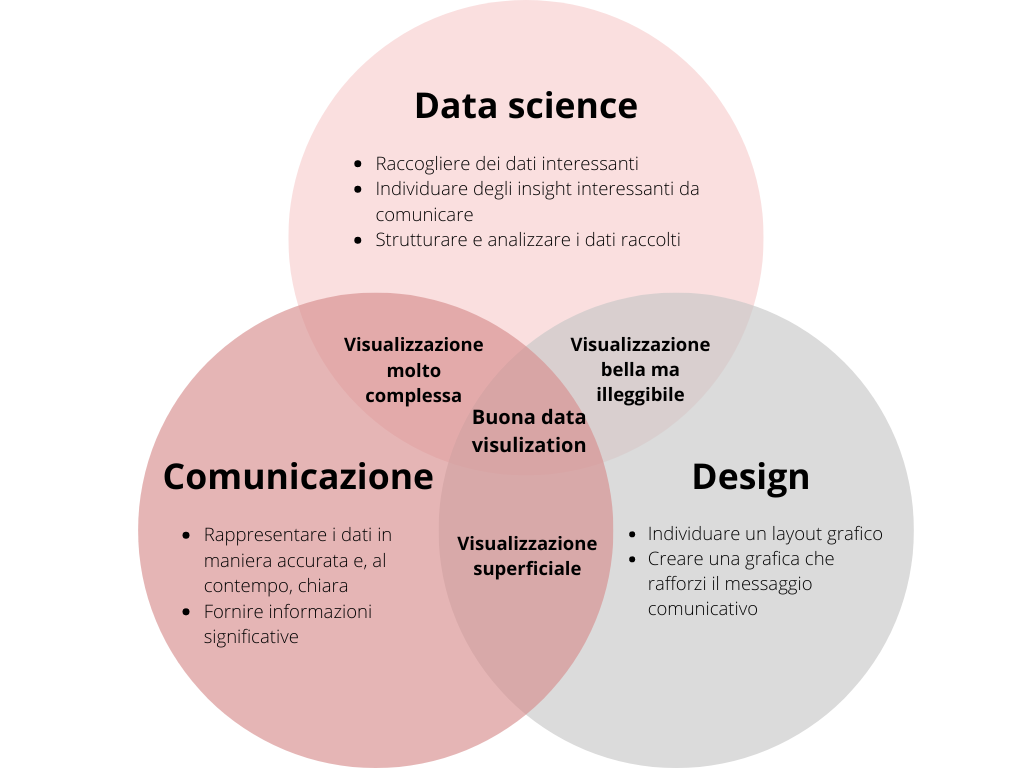
\includegraphics[width=0.8\columnwidth]{data-viz/venn_good_dataviz} 
    \caption{Diagramma di Venn: intersezione tra data science, comunicazione e design nella visualizzazione dei dati}
    \label{fig:venn_good_dataviz}
\end{figure}

\noindent Se realizzata correttamente, infatti, essa è capace di ricavare da \emph{dataset} complessi delle informazioni significative e trasmetterle in maniera intuitiva.
Usando le parole di Edward Tufte, statistico e luminare nel campo della \gls{datavizg}, una visualizzazione dei dati eccellente consiste in
``idee complesse comunicate con chiarezza, precisione ed efficienza''.
% TODO: aggiungere citazione come footnote (%“The visual Display of Quantitative Information” di Edward R. Tufte, CAP 1: Graphical excellence)

%cap1: “L'arte funzionale – Infografica e visualizzazione delle informazioni” di Alberto Cairo
Da ciò ne consegue che l'obiettivo della \gls{datavizg} e ruolo di un architetto dell'informazione è quello di rendere il più efficiente possibile il processo che il cervello
umano compie nell'acquisire conoscenza e saggezza a partire dall'osservazione di fenomeni.
Tale processo può essere descritto, in maniera semplificata, attraverso la cosiddetta gerarchia DIKV (\emph{Data-Information-Knowledge-Wisdom}) di seguito riportata.
\begin{figure}[!h] 
    \centering 
    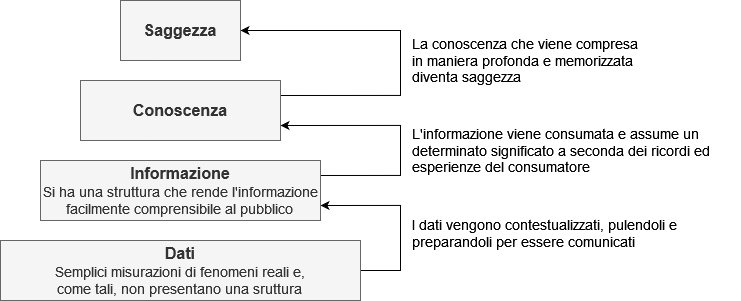
\includegraphics[width=\columnwidth]{data-viz/DIKV} 
    \caption{Gerarchia DIKV}
    \label{fig:DIKV}
\end{figure}

Come si nota subito dall'immagine \ref{fig:DIKV}, è essenziale ottenere dati puliti, completi e rappresentativi (responsabilità della \gls{datascienceg}). Solo successivamente sarà possibile rappresentare tali dati e 
ottenere una conoscenza valida (responsabilità di comunicazione e design).

\bigskip
%“L'arte funzionale – Infografica e visualizzazione delle informazioni” di Alberto Cairo
% cap 2
\noindent Nella visualizzazione dei dati in sé, bisogna tener conto innanzitutto che la forma grafica delle informazioni non è di per sé un'applicazione artistica; infatti, 
essa deve anche coadiuvare il fruitore in attività intellettive. Pertanto, la forma deve aspirare a oggettività, precisione e, soprattutto, funzionalità.
Per descrivere tale principio, possiamo dunque prendere in prestito le parole di Louis Sullivan sull'architettura modernista del XX secolo: ``La forma segue la funzione''. 
Tale massima può infatti essere applicata anche all'architettura dell'informazione nel contesto della \gls{datavizg}, giacché
un complesso di dati può assumere più forme, ma non tutte le forme sono sempre adatte e usabili. Infatti, la loro scelta deve dipendere dal
tipo di dati e obiettivo della rappresentazione. Ne consegue che più preciso è lo scopo, più limitata sarà la gamma di forme tra cui scegliere.

Il processo di decisione della rappresentazione grafica viene meglio approfondito nella sezione \ref{sec:classificare_grafici}.

\bigskip
\noindent Una volta decisa la forma migliore, bisogna comunque adattarla alla visualizzazione del caso specifico attraverso delle scelte di design.
In tal senso, si può adottare un approccio più minimalistico, promosso dal sopracitato Edward Tufte, o un approccio più ``artistico'', 
sostenuto da Nigel Holmes, famoso grafico specializzato nel design delle informazioni.

%“The visual Display of Quantitative Information” di Edward R. Tufte
%CAP 1: Graphical excellence
Per Tufte è essenziale combinare una semplicità di design a complessità dei dati. Per lui, il fruitore della visualizzazione deve poter ricavare il maggior numero di idee e informazioni dal minor uso possibile di spazio e inchiostro.
A tal proposito, egli sviluppa le seguenti formule: 
\begin{center}
    $\text{Rapporto dati-inchiostro} = \frac{\text{inchiostro usato per la codifica dei dati}}{\text{inchiostro totale usato per la stampa del grafico}}$
\end{center}
\begin{center}
    $\text{Densità dei dati} = \frac{\text{numero di voci in una matrice di dati}}{\text{area occupata dal grafico}}$            %CAP 8: Data density and small multiples
\end{center}
% TODO: aggiungere footnote che questa parte si intende solo quella dei datiDensità = number entries in una matrice di dati / area del grafico.
%Meglio se è più alta (mappe è altissima), risulta anche essere più affidabile. Bisogna comunque evitare di sovrappopolare lo spazio, in quel caso conviene utilizzare tecniche di data-reduction (averaging, clustering, smoothing).
%Attenzione! Stiamo parlando della parte di dati, per quanto riguarda la parte non strettamente riguardante questi (chartjunk) meglio meno.
evidenziando che più il rapporto è alto, migliore è la rappresentazione. Ciò implica che sia necessario evitare di utilizzare tutti gli elementi decorativi o, più in generale, tutte le parti che possono essere omesse 
senza perdere dati, ovvero tutto ciò che Tufte chiama \gls{chartjunkg} (e.g. la maggior parte delle griglie e sfondi posti sotto i grafici).

%“L'arte funzionale – Infografica e visualizzazione delle informazioni” di Alberto Cairo
%cap 3
D'altra parte, Holmes sostiene che ci si può divertire con la forma, purché la funzione principale rimanga comunicare i dati. Infatti, ciò che Tufte potrebbe considerare \gls{chartjunkg}, e dunque superfluo,
potrebbe invece rivelarsi utile al processo di memorizzazione e dunque portare più facilmente alla saggezza. 

%“L'arte funzionale – Infografica e visualizzazione delle informazioni” di Alberto Cairo
%Cap 4
Qualsiasi approccio si decida di intraprendere, rimane comunque essenziale sfruttare lo spazio a disposizione per ricercare la profondità, seppur rimanendo nei limiti dettati dal tipo di fruitori.
Tale profondità si concretizza quasi sempre tramite la rappresentazione di dati multivariati, che consentono l'analisi di un fenomeno in maniera più accurata. %multivariato da %“The visual Display of Quantitative Information” di Edward R. Tufte, CAP 1: Graphical excellence
Le informazioni non devono infatti essere semplificate o snellite dalla visualizzazione, bensì devono essere solamente chiarite. La rappresentazione dovrebbe permettere dunque di suscitare riflessioni non superficiali ed evidenziare tendenze, \emph{pattern} 
o fenomeni altrimenti invisibili. 
Solo in un secondo momento ci si può dedicare all'estetica della presentazione, utilizzando gli spazi rimanenti. Tale precauzione è da prendere affinché i dati ricevano subito tutto lo spazio necessario ed eventuali
effetti speciali o decorazioni siano inseriti solo se se ne presenta l'opportunità.


\subsection{Linee guida}
%“The visual Display of Quantitative Information” di Edward R. Tufte
%CAP 1: Graphical Integrity
Nel visualizzare dati è necessario garantire che le informazioni siano rappresentate accuratamente e senza distorsioni.
A tal scopo, è dunque necessario perseguire un'\textbf{integrità grafica}. Ciò implica l'uso di:
\begin{itemize}
    \item proporzioni corrette tra la rappresentazione dei numeri sul grafico e le quantità numeriche fornite, come pure tra il 
    numero di dimensioni rappresentate graficamente e il numero delle variabili nei dati;
    \item scale appropriate che mostrino la vera variazione dei dati (e.g. scale con intervalli regolari);
    \item etichette dettagliate e chiare che non fuorviino l'utente;
    \item elementi che contestualizzino il grafico.
\end{itemize}

%“The visual Display of Quantitative Information” di Edward R. Tufte
%CAP 9: AESTHETICS AND TECHNIQUE IN DATA GRAPHICAL DESIGN
\noindent Come accennato precedentemente, altrettanto importante è la \textbf{scelta del design}. Ciò include:
\begin{itemize}
    \item La scelta di un formato e \emph{layout} appropriato, scegliendo la combinazione di frasi, tabelle
    e grafici che meglio mostri la riflessione che si vuole comunicare (e.g. per più di due numeri, conviene usare una tabella piuttosto che una frase). Ciò comporta:
    \begin{itemize}
        \item per l'occidente, un orientamento (specie per quanto riguarda il testo) che va dall'alto a sinistra verso il basso a destra;
        \item l'uso di grafici corredati da piccoli messaggi di chiarimento, piuttosto che spiegazioni sparse.
    \end{itemize}
    \item L'uso simbiotico, coerente e diretto di parole, numeri e figure.
    \item Visualizzare i dati in maniera accessibile, anche e soprattutto per quanto riguarda dettagli di dati complessi. Ciò comporta:
    \begin{itemize}
        \item l'uso di codifiche non troppo elaborate, che non necessitino il continuo controllo della legenda;
        \item tenere in considerazione anche le persone daltoniche e \emph{color-deficient} nella scelta dei colori del grafico (se presenti);
        \item l'uso di caratteri leggibili.
    \end{itemize}
\end{itemize}



\section{Classificare i grafici}\label{sec:classificare_grafici}
Lo sviluppo e disponibilità al pubblico di nuovi strumenti avanzati ha consentito anche a utenti non esperti di visualizzare dati ed estrarne informazioni dettagliate, 
permettendo loro di creare grafici e diagrammi.
Tuttavia, persiste ancora un ampio divario di conoscenza tra questi utenti e i modelli visivi esistenti.
Ne consegue che spesso le forme visive scelte per la rappresentazione non sono le più efficaci essendo limitate da un ristretto numero di opzioni conosciute.
In alcuni casi, addirittura, la rappresentazione scelta risulta essere anche poco comprensibile o fuorviante per il caso d'uso specifico.

Senza una classificazione chiara, diventa dunque difficile per questo tipo di utenti selezionare la tecnica di visualizzazione più adeguata.
Nelle seguenti sezioni, si esaminano dunque dei criteri di classificazione identificati, assieme a uno strumento prototipale che mira ad 
automatizzare questo processo di classificazione.


\subsection{Metodo di classificazione}
I criteri principali da tenere in considerazione nella scelta del grafico sono:
\begin{itemize}
    \item l'obiettivo della visualizzazione,
    \item i tipi di dati disponibili.
\end{itemize}

\subsubsection{Obiettivi della visualizzazione}\label{subsubsec:obj}
Quando parliamo di ``obiettivo della visualizzazione'' intendiamo il tipo di relazione tra i dati che vogliamo mettere in evidenza attraverso
la rappresentazione grafica. I principali obiettivi individuati sono:
\begin{enumerate}
    \item \textbf{Divergenza}, quando si vogliono mettere in luce le differenze di valori a partire da un punto fisso (solitamente lo 0, ma può essere
    ad esempio anche una media).
    \begin{itemize}
        \item Esempio: confrontare la produttività del turno di giorno con quello del turno di notte.
    \end{itemize}
    \item \textbf{Correlazione}, quando si vuole enfatizzare la relazione tra due o più variabili. In questi casi, il fruitore della visualizzazione assumerà che le 
    variabili coinvolte siano in relazione causale, pertanto se così non fosse è necessario specificarlo.
    \begin{itemize}
        \item Esempio: esplorare come la qualità del sonno influenzi le prestazioni accademiche.
    \end{itemize}
    \item \textbf{\emph{Ranking}}, quando si vuole mostrare la posizione degli elementi rispetto agli altri e il loro valore effettivo passa in secondo piano.
    \begin{itemize}
        \item Esempio: mostrare i dieci paesi con il tasso di inquinamento più alto.
    \end{itemize}
    \item \textbf{Distribuzione}, quando si vogliono mostrare eventuali \emph{pattern} nei dati, evidenziando valori ed eventi di un \emph{dataset} e per quali casi essi si verificano. 
    \begin{itemize}
        \item Esempio: mostrare la frequenza di incidenti stradali per tipo di veicolo.
    \end{itemize}
    \item \textbf{Cambiamento nel tempo}, quando si vogliono enfatizzare dei \emph{trend} che variano nel tempo.
    \begin{itemize}
        \item Esempio: analizzare come l'uso dei social media è cambiato negli ultimi cinque anni.
    \end{itemize}
    \item \textbf{Composizione}, quando si vuole mostrare come una singola entità viene suddivisa nelle sue componenti.
    \begin{itemize}
        \item Esempio: mostrare la composizione delle emissioni di gas serra per settore industriale.
    \end{itemize}
    \item \textbf{Grandezze}, quando si vogliono comparare grandezze, che siano esse assolute (per un maggior livello di dettaglio) o relative. 
    \begin{itemize}
        \item Esempio: mostrare la dimensione del mercato degli smartphone in termini di volumi di vendita.
    \end{itemize}
    \item \textbf{Spazi}, quando si vogliono mostrare \emph{pattern} geografici o posizioni precise.
    \begin{itemize}
        \item Esempio: mostrare i paesi con la maggiore concentrazione di risorse naturali.
    \end{itemize}
    \item \textbf{Flussi}, quando si vogliono mostrare volumi o intensità del movimento/cambiamento tra due o più stati o condizioni.
    \begin{itemize}
        \item Esempio: esplorare la rete di interconnessioni finanziarie tra le banche.
    \end{itemize}
\end{enumerate}

\subsubsection{Tipi di dati}
Una prima distinzione nel tipo di dati riguarda:
\begin{itemize}
    \item \textbf{dati numerici},
    \item \textbf{dati categorici}.
\end{itemize}
Il \emph{dataset} fornito per la visualizzazione potrà dunque essere composto da dati tutti numerici, tutti categorici oppure da un mix dei due.

\bigskip
\noindent Un'altra distinzione si ha tra:
\begin{itemize}
    \item \textbf{dati univariati}, quando ho un \emph{dataset} molto piccolo composto da una sola variabile;
    \item \textbf{dati multivariati}, quando ho un \emph{dataset} composto da più variabili.
\end{itemize}

\bigskip
\noindent In base alle suddette classificazioni, si può specificare ulteriormente il tipo di dato:
\begin{itemize}
    \item In caso di \emph{dataset} con multiple variabili numeriche:
    \begin{itemize}
        \item \textbf{dati ordinati}, dove è presenta almeno una variabile numerica che è ordinata;
        \item \textbf{dati non ordinati}, dove l'ordine non è rilevante.
    \end{itemize}
    \item In caso di \emph{dataset} con multiple variabili categoriche:
    \begin{itemize}
        \item \textbf{organizzazione in sottogruppi}, una o più variabili categoriche specificano e rappresentano una sottopopolazione di un'altra variabile categorica;
        \item \textbf{organizzazione indipendente}, le variabili categoriche sono indipendenti tra di loro;
        \item \textbf{organizzazione gerarchica}, una o più variabili categoriche specificano un rapporto gerarchico rispetto ad un'altra variabile categorica padre.
    \end{itemize}
    \item In caso di almeno una variabile numerica e una categorica, con multiple variabili categoriche solo se organizzate in sottogruppi o in relazione gerarchica:
    \begin{itemize}
        \item \textbf{Una singola occorrenza}, quando a ogni individuo della popolazione, individuato dalle variabili categoriche, corrisponde un solo dato numerico;
        \item \textbf{Multiple occorrenze}, quando a ogni individuo della popolazione, individuato dalle variabili categoriche, corrispondono multipli valori numerici.
    \end{itemize}
\end{itemize}


\subsection{Chart-chooser}
%file criteri_scelta_grafico_v0.1.0 + codice + prompt LLM
%fonte: https://www.data-to-viz.com/ e https://ft-interactive.github.io/visual-vocabulary/
\emph{Chart-chooser} è uno strumento prototipale sviluppato nel corso dello stage che si serve del metodo di classificazione descritto 
nelle pagine precedenti per consigliare a un utente non esperto uno o più grafici che potrebbero rappresentare al meglio i dati disponibili.
Tale compito di classificazione viene gestito e realizzato principalmente tramite un \gls{sistemadiregoleg}, il cui funzionamento viene approfondito al paragrafo
\hyperref[subsubsec:rules]{Implementazione del sistema di regole}.

Lo strumento è disponibile a \href{http://www.overleaf.com}{questo link}.
% TODO: inserire link github 

\subsubsection{Analisi dei dati}
In primis, è necessario individuare il numero di variabili numeriche e categoriche presenti nel \emph{dataset}.
\emph{Chart-chooser} effettua tale processo in maniera semplificata, controllando se il primo valore per ogni variabile
è un numero (variabile numerica) o una stringa (variabile categorica).

Nel caso sia necessario, viene inoltre richiesto all'utente di rispondere ad alcune domande per chiarire ulteriori aspetti riguardanti il tipo 
di dato e individuare le ulteriori sotto-distinzioni (come descritte nella sezione precedente). Ad esempio, nel caso si abbiano dati multivariati numerici verrà chiesto 
se i dati sono ordinati o meno, mentre se si hanno dati univariati numerici non saranno necessarie ulteriori domande.

\subsubsection{Individuazione dell'obiettivo}
Una volta definito il tipo di dato è necessario individuare l'obiettivo della visualizzazione.
A tal fine, \emph{Chart-chooser} richiede all'utente di fornire una breve descrizione di ciò che vuole rappresentare e comunicare.
Il testo immesso viene poi elaborato da un \gls{llm}, il quale interpreta la descrizione e ne estrae l'obiettivo più pertinente tra i nove possibili (definiti e descritti in \ref{subsubsec:obj}). 
Come \gls{llm} viene utilizzato \textbf{\gls{llama7bg}} attraverso \textbf{\gls{llamacppg}}, reso disponibile dall'azienda ospitante. I parametri sono perlopiù quelli di default, tranne la temperatura che viene 
impostata a 0 per garantire che l'output del modello sia il più predicibile possibile e restituisca solamente il numero dell'obiettivo.

\bigskip
\noindent Per quanto riguarda invece il metodo di \gls{promptengg} utilizzato, si adopera una tecnica di \gls{fsl} implementata nello scenario dell'\gls{icl}.
Nello specifico, per ogni obiettivo vengono fornite al \gls{llm} alcune descrizioni d'esempio in modo tale da facilitare al modello il compito di classificazione e migliorarne le
prestazioni. Questo approccio permette al \gls{llm} di comprendere meglio il contesto e rispondere con una maggiore precisione.

Il prompt utilizzato è il seguente:
\begin{lstlisting}[style=htmlcssjs]
This is a conversation between User and Llama, a friendly chatbot. Llama is helpful, kind, honest, good at writing, and never fails to answer any requests immediately and with precision.

User: 
Dati i seguenti obiettivi:
Obiettivo 1: Mostrami la differenza tra i dati; Confronta due serie di dati divergenti; Mostrami la variazione rispetto a un valore.
Obiettivo 2: Mostrami un dato in relazione ad un altro; Mostrami come sono associati i due dati; Mostrami la correlazione tra un dato e i suoi due fattori.
Obiettivo 3: Mostrami la classifica; Mostrami i top; Mostrami i dati più importanti; Mostrami i più comuni; Mostrami i principali.
Obiettivo 4: Mostrami quante volte si verifica un evento; Mostrami la distribuzione del dato; Mostrami la media; Mostrami la frequenza.
Obiettivo 5: Mostrami la variazione nel tempo del dato; Mostrami la tendenza del dato nel tempo; Mostrami le differenze tra i dati nel tempo; Mostrami il cambiamento dei dati nel tempo; Mostrami le previsioni future.
Obiettivo 6: Mostrami i componenti del dato; Mostrami il dato diviso nei sottogruppi; Mostrami la struttura del dato; Mostrami la ripartizione del dato.
Obiettivo 7: Mostrami la dimensione effettiva del dato; Mostrami le unità; Mostrami la misura del dato; Mostra la rilevanza del dato all'interno di un contesto; Mostrami la grandezza dei dati.
Obiettivo 8: Mostrami la posizione; Mostrami i flussi nel mondo; Mostrami la mappa di distribuzione; Mostrami i paesi in cui si verifica l'evento; Mostrami la variazione nello spazio del dato.
Obiettivo 9: Mostrami i flussi tra i vari punti; Mostrami la rete; Mostrami le relazioni e la loro intensità; Mostrami cosa influisce nel dato; Mostrami come sono relazionati all'interno di un sistema. 

Classifica la seguente frase, dimmi solamente il numero dell'obiettivo senza altre parole: 
${descrizione_utente}
Llama:
\end{lstlisting}
% TODO: rivedere prompt su chart-chooser e inserire modello usato corretto (7b?)

\subsubsection{Implementazione del sistema di regole}\label{subsubsec:rules}
Le informazioni raccolte sono utilizzate da un \gls{motoreregoleg} per combinare le analisi e le classificazioni effettuate e restituire il nome dei possibili grafici applicabili al caso d'uso, se presenti.
Si precisa, infatti, che non per tutti gli obiettivi sono presenti tutti i tipi di dato. Pertanto, la combinazione potrebbe portare a un risultato nullo.

Il \gls{motoreregoleg} scelto è \textbf{\gls{jsonrulesg}}. Tale decisione è motivata dalla sua leggerezza e velocità, nonché dal fatto che le regole siano semplici strutture JSON, 
il che le rende più leggibili dall'uomo e facili da mantenere.

\bigskip
\noindent Gli elementi principali che caratterizzano tale sistema sono:
\begin{itemize}
    \item I \emph{fatti}, ovvero dei valori costanti o funzioni pure.
    \item Le \emph{regole}, ovvero delle strutture composte da:
    \begin{itemize}
        \item \emph{Condizioni}, nella forma \texttt{[fact: nome\_fatto, operator: tipo\_operatore, value: valore\_da\_controllare]}
        che rappresentano i ``requisiti'' della regola, soddisfatti se la relazione definita dall'operatore tra il valore del \emph{fatto} e il valore prestabilito 
        indicato risulta vera. Si precisa, inoltre, che possono essere creati insiemi di queste \emph{condizioni} attraverso l'uso di operatori booleani.
        \item \emph{Eventi}, ovvero delle operazioni che il \emph{motore} esegue in base al soddisfacimento o meno delle \emph{condizioni}. 
    \end{itemize}
    \item Il \emph{motore di inferenza} in sé, a cui vengono dati in input i \emph{fatti} e aggiunte le \emph{regole}. Esso è il cuore del \gls{motoreregoleg} in quanto si occupa di valutare
    le \emph{regole} basandosi sui \emph{fatti} forniti, innescando \emph{eventi} a seguito del soddisfacimento o meno delle \emph{condizioni}.
\end{itemize}
%TODO: inserire codice esempio cose

\bigskip
\noindent Per quanto riguarda il funzionamento specifico di ``Chart-chooser'', si hanno come \emph{fatti} iniziali solamente il numero di variabili numeriche e categoriche. 
Per quanto riguarda gli altri \emph{fatti}, che richiedono un input da parte dell'utente (e.g. l'obiettivo o il fatto di essere dati numerici ordinati o meno), questi sono 
forniti al \emph{motore} durante la sua esecuzione all'innescarsi di determinati \emph{eventi}. 
Ciò permette di poter valutare subito le regole sui \emph{fatti} già noti e nel frattempo poter ottenere dall'utente il valore dei rimanenti, fermando eventualmente l'esecuzione del \emph{motore} solo
prima di regole che necessitano dei \emph{fatti} ancora sconosciuti. % TODO: ottenere come promise?
In tale maniera, inoltre, vengono richiesti all'utente e forniti al \emph{motore} solamente i \emph{fatti} che concernono la situazione specifica. Ad esempio, nel caso in cui si abbiano solamente dati numerici, 
non verrà chiesta all'utente e non sarà fornita inutilmente al \emph{motore} l'informazione riguardante l'organizzazione delle variabili categoriche.

Tale funzionamento è possibile grazie alla definizione di un \gls{sistemadiregoleg} basato sulle \emph{priorità}, le quali determinano l'ordine di esecuzione delle \emph{regole} stesse.
Nello specifico, una \emph{priorità} maggiore comporta una valutazione anticipata; mentre, in caso di uguale \emph{priorità} tra più \emph{regole}, queste verranno valutate in parallelo.
Ne consegue che le \emph{regole} allo stesso livello di \emph{priorità} servano a identificare le classificazioni relative a un determinato tema e presentano dunque \emph{condizioni} mutualmente esclusive.
Il soddisfacimento delle \emph{condizioni} di una di queste \emph{regole} viene poi comunicato al livello inferiori di \emph{priorità}, aggiungendolo ai \emph{fatti}, in modo tale che solamente le \emph{regole} che richiedono
tale \emph{condizione} siano passabili.


Si ha dunque il seguente \gls{sistemadiregoleg}:
%TODO: albero regole



%\subsubsection{Proposta di grafici}
%Dopo un attento studio dei grafici e metodi di classificazioni trovati.
%TODO inserire fonti, capire cosa scrivere

%Tecnologie utilizzate

\subsubsection{Limitazioni dello strumento}
Come già accennato precedente \emph{Chart-chooser} è uno strumento prototipale, presenta infatti diverse limitazioni.
Innanzitutto, l'applicativo è disponibile soltanto da console e non dispone di un'interfaccia grafica.
%TODO: numerici categorici boh date, presuppone conoscenza dell'utente sul set di dati (essendo che chiedo domande)
%file disponibile in locale e di tipo json costruito in un certo modo
%TODO: per un futuro approfondire parsing dati
    \chapter{Infografiche}
\label{cap:studio_infografiche}
\intro{In questo capitolo verranno esaminate le caratteristiche funzionali e di design delle infografiche e 
presentate le loro applicazioni. Verrà inoltre fornita una classificazione delle infografiche basata sulla 
loro struttura e output visivo.}\\

\section{Definizione e applicazioni}
\subsection{Cos'è un infografica e in cosa si distingue dalla data visualization}
%cap1: Design della mente – infografica e data viz” di Paolo Bottazini, Michele Gotuzzo 
Analogamente alla \gls{datavizg}, le infografiche si occupano di rappresentare visivamente i dati al fine di comunicarli in maniera più semplice e accessibile.
Esse trasformano i dati in idee chiare, permettendo di inquadrare facilmente un fenomeno, una situazione o un processo, coadiuvando così la presa di decisioni ponderate sul tema presentato.
Queste idee sono generate a partire dall'interpretazione, formalizzazione e contestualizzazione dei dati, che spesso sono disomogenei per formato, tipo di contenuto e origine. Tale interpretazione ha il compito di 
svelare il significato nascosto nel \emph{dataset} e selezionare le connessioni o fenomeni più interessanti per il destinatario della comunicazione.
In altre parole, l'infografica non si limita a mostrare i dati, ma li organizza e li presenta in un modo da renderne più evidente significato e importanza.

Per raggiungere questo obiettivo, le infografiche combinano elementi testuali e grafici per presentare le informazioni; usando le parole di E. Tufte ``un'infografica mostra visivamente grandezze misurate mediante 
l'uso combinato di punti, linee, un sistema di coordinate, numeri, simboli, parole, ombreggiature e colore''. Pertanto, le infografiche rigettano la tradizione di ``purezza grafica'' (i.e. rappresentazione dei dati 
basata solo su grafici, diagrammi e mappe) imposta alla \gls{datavizg} e abbracciano, invece, un insieme molto più amplio di tecniche di comunicazione visiva, come illustrazioni, immagini, etc.
% TODO: aggiungere citazione come footnote The visual display of quantitative information, Edward Tufte [2001], Introduction, p.10
Inoltre, il focus dell'infografica non è solamente l'oggetto da rappresentare, come invece accade con la \gls{datavizg}. Infatti, le infografiche
prendono in considerazione anche il destinatario della comunicazione, scegliendo e disponendo gli elementi per costruire una narrazione.
Possiamo infatti pensare all'infografica come a una forma di racconto, di lettura che non è di per sé né imparziale né completa, ma si limita a fare luce ed esporre i punti salienti individuati nel \emph{dataset}.
%intro: “L'arte funzionale – Infografica e visualizzazione delle informazioni” di Alberto Cairo
In realtà, tale caratteristica delle infografiche è proprio ciò che maggiormente le distingue dalla \gls{datavizg}. Infatti, mentre le prime sono progettate per presentare i dati raccontandoli attraverso storie specifiche, guidando il lettore con una narrazione, la seconda
è più orientata verso l'esplorazione autonoma delle informazioni da parte del fruitore, che deve analizzare e scoprire i dati per conto proprio. 
Questa differenza nel livello di analisi richiesto si ripercuote anche sul tipo di pubblico di ciascun tipo di rappresentazione. Nello specifico, le infografiche, grazie alla loro capacità di semplificare e contestualizzare i dati, sono accessibili anche a coloro
che non possiedono capacità analitiche avanzate e, pertanto, hanno un pubblico più ampio. 

%intro: “L'arte funzionale – Infografica e visualizzazione delle informazioni” di Alberto Cairo
Nonostante queste differenze, infografiche e \gls{datavizg} sono strettamente connesse e complementari. Le infografiche, pur essendo maggiormente orientate alla narrazione, 
possono includere elementi che stimolano l'esplorazione autonoma dei dati. Allo stesso modo, le \emph{visualizzazioni dei dati} possono contenere aspetti narrativi che facilitano 
l'interpretazione.


\subsection{Applicazioni e vantaggi}
Le infografiche sono strumenti versatili che vengono utilizzati in una vasta gamma di settori e contesti, in particolare al fine 
di analizzare o presentare dati. Offrono infatti vantaggi significativi che le rendono particolarmente adatte a questi scopi.

%Infographics: The New Communication Tools in Digital Age, Waralak V. Siricharoen
Per quanto riguarda l'\textbf{analisi dei dati}, le infografiche sono utili per la cosiddetta \gls{expdataanalysisg}, dove il fruitore non ha una domanda precisa a cui sta cercando risposta, bensì 
vuole semplicemente scoprire cosa emerge di interessante dal \emph{dataset}.

Per quanto riguarda invece la \textbf{presentazione dei dati}, va da sé che le infografiche siano perfette per tale scopo, in quanto riescono attraverso una narrazione a comunicare in maniera efficace 
e abbracciare in tal modo un pubblico molto amplio.

\bigskip
\noindent In generale, quale sia l'applicazione, l'uso di infografiche consente anche di:
\begin{itemize}
    \item \textbf{Facilitare la scoperta di informazioni} nascoste e \textbf{stimolare la curiosità} per una ricerca futura;
    \item \textbf{Semplificare la comprensione}, facilitando così il raggiungimento della \emph{saggezza};
    \item \textbf{Raccontare una storia} che permetta una visione d'insieme della situazione, fenomeno o processo presentato.
\end{itemize}



\section{Classificare le infografiche}
\subsection{Metodi di classificazione}\label{subsec:info_classifica}
% file criteri_scelta_infografica_v0.1.0
Una prima classificazione delle infografiche può essere fatta \textbf{in base all'output visivo}. Nello specifico, si hanno:
\begin{itemize}
    \item \textbf{Infografiche statiche}, in cui le informazioni sono rappresentate e visibili tutte in un'unica volta, avendo così un impatto più
    veloce e immediato sul pubblico.
    \begin{itemize}
        \item Esempio: infografiche presenti nei giornali.
    \end{itemize}
    \item \textbf{Infografiche animate}, in cui le informazioni sono presentate sequenzialmente in maniera consistente oppure contengono altri tipi di animazione.
    \begin{itemize}
        \item Esempio: infografiche realizzate tramite presentazioni multimediali.
    \end{itemize}
    \item \textbf{Infografiche interattive}, in cui le informazioni sono presentate in base a scelte operate dall'utente.
    \begin{itemize}
        \item Esempio: infografiche online in cui è l'utente a selezionare il dettaglio a partire da un insieme complesso di informazioni visualizzate.
    \end{itemize}
\end{itemize}

\bigskip
\noindent Un'altra classificazione può essere fatta \textbf{in base all'obiettivo}. Nello specifico, si hanno:
\begin{itemize}
    \item \textbf{Infografiche basate su processi ordinati}, le quali vengono usate per mostrare passo dopo passo un processo o una 
    sequenza ordinata di informazioni ad esempio per insegnare qualcosa di nuovo all'utente (e.g. ricette).
    \item \textbf{Infografiche a mo' di lista}, in questo caso le informazioni sono rappresentate sotto forma di elenco testuale, eventualmente accompagnato da icone.
    Per costruzione, queste infografiche permettono di mostrare molte informazioni e, allo stesso tempo, di farle comprenderle velocemente.
    \item \textbf{Infografiche basate sul tempo}, in cui viene mostrata una sequenza cronologica di eventi, in altre parole come si evolve una storia o un soggetto nel tempo.
    Quest'ultimo è solitamente rappresentato tramite una linea, chiamata appunto ``linea del tempo''.
    \item \textbf{Infografiche basate sul confronto}, esse comparano due diversi argomenti in contrasto ponendoli uno a fianco all'altro.  Ciò ritorna molto utile per mostrare
    quali elementi i due hanno in comune oppure per quanto divergono o sono superiori/inferiori uno rispetto all'altro.
    \item \textbf{Infografiche basate su una gerarchia}, le quali vengono utilizzate per mostrare informazioni organizzate per livelli e il collegamento tra questi.
    \item \textbf{Infografiche basate su informazioni correlate poste allo stesso livello}, in cui si vuole comunicare un nuovo concetto o dare una panoramica su un argomento; infatti,
    tali infografiche sono anche dette ``Infografiche informative''. Solitamente, lo spazio viene diviso in sezioni con un proprio titolo descrittivo.
\end{itemize}


\subsection{Infographic-helper}
Come accennato in precedenza, l'infografica è una forma di racconto e, pertanto, la scelta e scrittura della storia da comunicare sono centrali nella sua costruzione.
Nel corso dello stage si è dunque voluto sviluppare uno strumento prototipale, \emph{Infographic-helper}, che potesse aiutare il ``narratore'' in tale compito.
Nello specifico, questo strumento consente di validare tale narrativa, oltre a individuarne le parti e l'obiettivo principale.

Lo strumento è disponibile a \href{http://www.overleaf.com}{questo link}.

\subsubsection{Validazione della narrativa}
Uno degli obiettivi di \emph{Infographic-helper} è garantire che la narrativa dell'infografica sia persuasiva e venga recepita efficacemente dal pubblico. 
Questi obiettivi coincidono con quelli della retorica, la quale fornisce i principi per costruire messaggi convincenti e chiari, che espongono il punto di vista del comunicatore in maniera comprensibile. 
Questi principi non solo sono applicabili alla pura comunicazione verbale, ma si rivelano utili anche per le infografiche. 
Infatti, nonostante queste siano rappresentazioni visive, esse sono comunque una forma di narrazione e comunicazione e pertanto oggetto di retorica. 

Aristotele, pioniere di quest'arte, definisce suddetti principi come \emph{ethos}, \emph{pathos} e \emph{logos}. Nello specifico:
\begin{itemize}
    \item \textbf{\emph{Ethos}}, comprende tutto ciò che stabilisce o aumenta la credibilità e autorità del comunicatore e delle fonti;
    \item \textbf{\emph{Pathos}}, comprende tutto ciò che suscita emozioni nel pubblico, che crea una connessione emotiva con gli spettatori;
    \item \textbf{\emph{Logos}}, comprende tutto ciò che fa parte di un'argomentazione razionale, logica e coerente, come dati e statistiche.
\end{itemize}
\emph{Infographic-helper} si ispira dunque a questi principi aristotelici per migliorare la costruzione delle storie delle infografiche. Nello specifico, controlla che questi elementi siano presenti
nel testo e, eventualmente, ne suggerisce di altri.

In aggiunta a questi elementi retorici, \emph{Infographic-helper} tiene conto anche del target dell'infografica, ovvero il pubblico a cui è destinata, per poter contestualizzare meglio la storia. 
Inoltre, lo strumento controlla anche se sono presenti eventuali elementi estranei o irrilevanti per il tema principale della storia. 

\bigskip
\noindent Queste funzionalità sono implementate attraverso interrogazione a un \gls{llm}, nello specifico un modello a 7 miliardi di parametri, utilizzato attraverso \textbf{\gls{llamacppg}} e reso disponibile dall'azienda ospitante.

Il \emph{prompt} utilizzato è il seguente:
\begin{lstlisting}[style=htmlcssjs]
Questa è una conversazione tra User e Llama, un chatbot amichevole. Llama è disponibile, onesto, bravo a scrivere e non manca mai di rispondere immediatamente e con precisione a qualsiasi richiesta.

User: 
Devo presentare il seguente testo a ${target}.
${ethos}.

Testo:
${storia}

Domande:
1.	Supponi che un elemento è di 'pathos' se può indurre il pubblico a sentire (o non sentire) una connessione emotiva con il contenuto.
    Riporta tutti gli elementi (frasi, espressioni e parole) di 'pathos' del Testo, SOLO se hanno senso nel contesto del Testo. Suggerisci altre frasi incisive di 'pathos' da poter inserire nel Testo.
2.  Supponi che un elemento è di 'ethos' se può indurre il pubblico a ritenere che l'autore sia (o meno) affidabile e credibile.
    Riporta tutti gli elementi (frasi, espressioni e parole) di 'ethos' del Testo, SOLO se hanno senso nel contesto del Testo. Suggerisci altre frasi incisive di 'ethos' da poter inserire nel Testo basandoti sul mio ruolo SE rilevante al tema del Testo.
3.  Supponi che un elemento è di 'logos' se può indurre il pubblico a credere che l'argomentazione sia (o meno) logica e supportata da prove adeguate.
    Riporta tutti gli elementi (frasi, espressioni e parole) di 'logos' del Testo, SOLO se hanno senso nel contesto del Testo. Suggerisci altre frasi incisive di 'logos' da poter inserire nel Testo.
4.	Supponi che un elemento è 'estraneo' se può ritenersi estraneo rispetto al tema principale del Testo oppure può ritenersi un'assurdità.
    Riporta tutti gli elementi (frasi, espressioni e parole) 'estraneo' presenti nel Testo.

[...continua...]
\end{lstlisting}
% TODO: inserire modello usato corretto (7b?) e llama.cpp
dove \texttt{\$target} rappresenta il pubblico di destinazione dell'infografica e \texttt{\$ethos} rappresenta il ruolo di chi espone la storia, inseriti per una maggiore contestualizzazione della storia poi riportata (inserita al posto di \texttt{{\$storia}}).

\subsubsection{Ricerca del layout da utilizzare}
L'altro obiettivo di \emph{Infographic-helper} è quello di classificare la storia in base alla seconda classificazione data in \ref{subsec:info_classifica} (ovvero la ``classificazione per obiettivo'') e trovare le sue principali parti costitutive.
Tali informazioni consentono di individuare il \emph{layout} più adatto per raccontare visivamente la storia e definire l'argomento specifico da trattare per ciascuna delle sezioni di tale \emph{layout}.

I possibili \emph{layout} sono descritti al paragrafo \ref{subsec:info_layout}.

\bigskip
\noindent Queste funzionalità sono anch'esse implementate attraverso interrogazione al \gls{llm} descritto precedentemente. 

Il \emph{prompt} utilizzato è il seguente:
\begin{lstlisting}[style=htmlcssjs]
[...segue...]
5.	Quali sono le parti in cui si divide il testo? Per ogni parte, dimmi solo un titoletto breve.
6.	Tolta l'introduzione, identifica la relazione generale tra le parti come una delle seguenti:
    -	parti di una lista, 
    -	parti di una linea del tempo, 
    -	parti poste a confronto, 
    -	parti che compongono gerarchia, 
    -	parti correlate poste allo stesso livello, 
    -	parti di un processo ordinato. 

Fornisci solamente le risposte nel seguente formato JSON: 
{ 'pathos': { 'presente': boolean, 'elementi': [string], 'suggerimenti': [string] }, 'ethos': { 'presente': boolean, 'elementi': [string], 'suggerimenti': [string] }, 'logos': { 'presente': boolean, 'elementi': [string], 'suggerimenti': [string] }, 'elementi_estraneo': {'presente': boolean, 'elementi': [string]}, 'parti': [string], 'relazione': 'string' }


Llama:
\end{lstlisting}

\noindent Si noti inoltre che è stata definita una \gls{grammaticag} corrispondente allo schema menzionato nel prompt (fornito per ulteriore chiarezza), la quale consente di ottenere l'output del \gls{llm} nel formato fisso \gls{jsong} indicato. 
Questo approccio facilita il \emph{parsing} dei dati, garantendo risposte precise con un formato standard, e ne agevola l'eventuale integrazione futura con un'interfaccia grafica.


\subsubsection{Limitazioni dello strumento}
Come già accennato precedentemente \emph{Infographic-helper} è uno strumento prototipale, presenta infatti diverse limitazioni.
Innanzitutto, l'applicativo è disponibile soltanto da riga di comando e non dispone di un'interfaccia grafica.
Inoltre, esso non ha la capacità di individuare molteplici obiettivi. Potrebbero essere infatti presenti diverse macro-sezioni nella narrativa
con obiettivi distinti. 
Lo strumento, inoltre, non è capace di valutare la veridicità del contenuto della storia, ma valida soltanto il modo in cui questo è comunicato. Pertanto, è compito dell'utente
assicurarsi che quanto scritto corrisponda a verità.

Ciononostante, \emph{Infographic-helper} ha il potenziale per essere migliorato e offrire un'esperienza utente più semplice e intuitiva.
%TODO: aggiungere che fa schifo ?, aggiungere parti test ?



\section{Design delle infografiche}
\subsection{I fattori che influenzano il design}
Possiamo ordinare gerarchicamente i fattori che influenzano la struttura del design delle infografiche. Tale gerarchia è suddivisa in sei livelli come segue:
%TODO: inserire da dove presa img, optimization of ....
\begin{figure}[H] 
    \centering 
    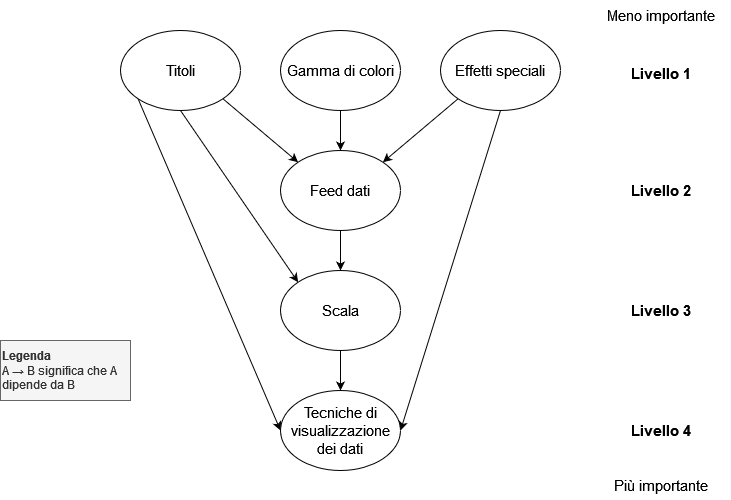
\includegraphics[width=0.8\columnwidth]{infografiche/fattori_design_info.png} 
    \caption{Gerarchia dei fattori che influenzano il design delle infografiche}
    \label{fig:fattori_design_info}
\end{figure}
\noindent Vediamo dunque come applicare al meglio tali fattori nella costruzione del design di un'infografica.

\subsubsection{I colori}
%“Design della mente – infografica e data viz” di Paolo Bottazini, Michele Gotuzzo
%CAP 16: Il colore
Il colore è un elemento cruciale nel design delle infografiche e, pertanto, è da utilizzare con cura. 
Esso infatti, se scelto in maniera appropriata, può migliorare la leggibilità e facilitare la comprensione e memorizzazione dell'informazione.

Generalmente, si utilizza il colore per catturare l'attenzione, evidenziare dati specifici e per rafforzare il messaggio narrativo. Quest'ultimo punto, in particolare, è possibile in quanto ogni colore porta con sé un 
significato simbolico influenzato dalla cultura e dalla geografia che permette di evocare sensazioni e valori specifici nel pubblico.
Di seguito sono riportati i valori più spesso associati ai colori, con riferimento alla cultura dell'Occidente:
\begin{itemize}
    \item Colori caldi:
    \begin{itemize}
        \item \textbf{Rosso}:
        \begin{itemize}
            \item Valori: emozioni forti come amore o aggressività.
            \item In linea con tali valori, viene utilizzato principalmente per attirare l'attenzione.
        \end{itemize}
        \item \textbf{Arancione}:
        \begin{itemize}
            \item Valori: ottimismo, vitalità.
            \item In linea con tali valori, viene generalmente utilizzato per temi giovanili e/o dinamici.
        \end{itemize}
        \item \textbf{Giallo}:
        \begin{itemize}
            \item Valori: energia, allegria, felicità.
            \item In linea con tali valori, viene anch'esso utilizzato principalmente per attirare l'attenzione, specie per temi innovativi.
        \end{itemize}
    \end{itemize}
    \item Colori freddi:
    \begin{itemize}
        \item \textbf{Verde}:
        \begin{itemize}
            \item Valori: salute, natura, tranquillità.
            \item In linea con tali valori, viene generalmente utilizzato per temi riguardanti la sanità, salute ed ecologia.
        \end{itemize}
        \item \textbf{Blu}:
        \begin{itemize}
            \item Valori: affidabilità, sicurezza, stabilità.
            \item In linea con tali valori, viene utilizzato ad esempio da banche o compagnie assicurative.
        \end{itemize}
        \item \textbf{Viola}:
        \begin{itemize}
            \item Valori: eleganza, nobiltà, spiritualità.
            \item In linea con tali valori, viene generalmente utilizzato per temi riguardanti il settore della bellezza o del lusso.
        \end{itemize}
    \end{itemize}
    \item Colori neutri:
    \begin{itemize}
        \item \textbf{Marrone}:
        \begin{itemize}
            \item Valori: terra, calore.
            \item In linea con tali valori, viene generalmente utilizzato per temi riguardanti la natura.
        \end{itemize}
        \item \textbf{Bianco}:
        \begin{itemize}
            \item Valori: purezza, pulizia, semplicità.
            \item In linea con tali valori, viene generalmente utilizzato per temi riguardanti la sanità.
        \end{itemize}
        \item \textbf{Nero}:
        \begin{itemize}
            \item Valori: ribellione, formalità, potenza.
            \item In linea con tali valori, viene generalmente utilizzato per temi di protesta o riguardanti il settore del lusso.
        \end{itemize}
        \item \textbf{Grigio}:
        \begin{itemize}
            \item Valori: modernità, raffinatezza.
            \item In linea con tali valori, viene generalmente utilizzati per temi riguardanti tecnologia o moda.
        \end{itemize}
    \end{itemize}
\end{itemize}

\bigskip
\noindent In ogni caso, è fondamentale mantenere un tono di colore coerente nell'infografica, preferibilmente tonalità sobrie. Tuttavia, potrebbe essere utile adoperare colori 
complementari per trasmettere sensazioni di calma oppure combinazioni di colori più stridenti per rappresentare innovazione.

Si aggiunge infine che, come per la \gls{datavizg}, anche in questo caso, è importante scegliere una gamma di colori che sia accessibile anche a persone daltoniche o \emph{color-deficient}.

\subsubsection{I layout}\label{subsec:info_layout}
% “Visual doing” di Willemien Brand 
Gli elementi di un'infografica possono essere disposti in un massimo di sei livelli:
\begin{itemize}
    \item Il \textbf{titolo principale};
    \item Il \textbf{sottotitolo};
    \item Il \textbf{contenuto principale e secondario};
    \item Gli \textbf{elementi di supporto}, come ad esempio divisori, contenitori etc.
    \item Gli \textbf{elementi di dettaglio}, come ad esempio le note a margine;
    \item I \textbf{comandi} di interazione e gli \textbf{\emph{highlights}} dei dati.
\end{itemize}

\bigskip
% Acquired Codes of Meaning in Data Visualization and Infographics: Beyond Perceptual Primitives, Lydia Byrne, Daniel Angus, and Janet Wiles
\noindent Per quanto riguarda nello specifico la struttura del contenuto principale e secondario, le infografiche sono solite
utilizzare una ``composizione a \emph{panel}'', ovvero si hanno diverse componenti grafiche, dette \emph{gruppi visivi}, leggibili in sequenza.
Questo approccio differisce notevolmente dalle pratiche comunemente usate nella \gls{datavizg}, dove tutte le sfaccettature del tema d'interesse sono presentate 
in un'unica composizione grafica.

La direzione e ordine in cui questa sequenza di \emph{gruppi visivi} viene presentata all'interno dell'infografica dipende dalla 
storia che si vuole raccontare. Infatti, per trasmettere efficacemente le informazioni e la narrativa, è necessario avere una struttura semantica sottostante all'infografica
che collega i \emph{gruppi visivi} in una determinata maniera dipendente dal messaggio. Questa struttura è detta \gls{vif}, letteralmente ``flusso delle informazioni visive''.
Tale flusso è spesso rimarcato ed evidenziato tramite l'uso di ``suggerimenti narrativi'', che possono essere espliciti, come frecce o descrizione testuali, oppure impliciti, se 
provengono da vari principi di design come ad esempio i principi di \emph{Gestalt} (approfonditi alla sezione \ref{subsec:gestalt}).
%TODO: studi di ... che analizzano vif nei vari hanno permesso di individuare pattern

Sono individuati i seguenti \emph{pattern} principali di \gls{vif}, distinti in base alla loro \emph{backbone shape}, ovvero da una diversa forma della linea lungo cui la 
maggior parte dei \emph{gruppi visivi} è allineata nella narrazione.
\begin{table}[H]
    \centering
    \begin{tabular}{|>{\centering\arraybackslash} m{0.15\columnwidth}| >{\centering\arraybackslash} m{0.25\columnwidth}| >{\centering\arraybackslash} m{0.15\columnwidth}| >{\centering\arraybackslash} m{0.25\columnwidth}|}
        \hline
        \rowcolor{gray!20}
        \textbf{Backbone Shape} & \textbf{Pattern} & \textbf{Backbone Shape} & \textbf{Pattern} \\
        \hline
        \begin{center}
\includegraphics[width=0.08\textwidth]{infografiche/clock_vif.png}\end{center} & Clock 
        & \begin{center}
\includegraphics[width=0.08\textwidth]{infografiche/downladder_vif.png}\end{center} & Down-ladder \\
        \begin{center}
\includegraphics[width=0.08\textwidth]{infografiche/dome_vif.png}\end{center} & Dome
        & \begin{center}
\includegraphics[width=0.08\textwidth]{infografiche/upladder_vif.png}\end{center} & Up-ladder \\
        \begin{center}
\includegraphics[width=0.08\textwidth]{infografiche/bowl_vif.png}\end{center} & Bowl
        & \begin{center}
\includegraphics[width=0.08\textwidth]{infografiche/landscape_vif.png}\end{center} & Landscape \\
        \begin{center}
\includegraphics[width=0.08\textwidth]{infografiche/leftwing_vif.png}\end{center} & Left-wing 
        & \begin{center}
\includegraphics[width=0.08\textwidth]{infografiche/portrait_vif.png}\end{center} & Portrait \\
        \begin{center}
\includegraphics[width=0.08\textwidth]{infografiche/rightwing_vif.png}\end{center} & Right-wing
        & \begin{center}
\includegraphics[width=0.08\textwidth]{infografiche/pulse_vif.png}\end{center} & Pulse \\
        \begin{center}
\includegraphics[width=0.08\textwidth]{infografiche/star_vif.png}\end{center} & Star 
        & \begin{center}
\includegraphics[width=0.08\textwidth]{infografiche/spiral_vif.png}\end{center} & Spiral \\
        \hline
    \end{tabular}
    \vspace{0.2cm}
    \caption{Backbone shape dei pattern di Visual Information Flow (VIF)}
    \label{tab:pattern_vif}
\end{table}

\noindent Le informazioni, dunque, saranno disposte all'interno dell'infografica a seconda dell'obiettivo della storia da raccontare.
Per la definizione degli obiettivi si rimanda alla sezione \ref{subsec:info_classifica}.

Nello specifico, vengono definite le seguenti disposizioni generali a cui si possono facilmente far corrispondere i diversi \emph{pattern} di \gls{vif} sopraelencati. 
% “Visual thinking” di Willemien Brand 
\begin{itemize}
    \item Disposizione \textbf{a lista}:
    \begin{itemize}
        \item Applicazione: come suggerisce il nome è adatta a infografiche che hanno come obiettivo rappresentare un elenco (e.g. orari o programmi), ma 
        anche infografiche basate su una gerarchia.
        \item Direzione: la storia viene presentata a partire dall'alto verso il basso. In alcuni casi, potrebbe anche essere orientata da sinistra verso destra.
        \item \emph{Pattern} \gls{vif}:
        \begin{itemize}
            \item \textbf{Portrait};
            \item \textbf{Landscape};
            \item \textbf{Down-ladder}. 
        \end{itemize}
    \end{itemize}
    \item Disposizione \textbf{a passi}:
    \begin{itemize}
        \item Applicazione: per infografiche che rappresentano processi ordinati.
        \item Direzione: la storia viene presentata dal basso verso l'alto e/o seguendo un percorso a zigzag che parte da sinistra e, generalmente, termina al lato opposto.
        \item \emph{Pattern} \gls{vif}:
        \begin{itemize}
            \item \textbf{Pulse};
            \item \textbf{Spiral};
            \item \textbf{Up-ladder}. 
        \end{itemize}
    \end{itemize}
    \item \textbf{\emph{Timeline}}:
    \begin{itemize}
        \item Applicazione: per infografiche basate sul tempo.
        \item Direzione: la storia viene presentata da sinistra verso destra oppure dall'alto verso il basso, solitamente avendo come riferimento una singola linea rappresentante il tempo.
        \item \emph{Pattern} \gls{vif}:
        \begin{itemize}
            \item \textbf{Portrait};
            \item \textbf{Landscape}.
        \end{itemize}
    \end{itemize}
    \item Disposizione \textbf{a mandala}:
    \begin{itemize}
        \item Applicazione: per infografiche basate su informazioni correlate poste allo stesso livello.
        \item Direzione: la storia si sviluppa dal centro verso l'esterno, seguendo un \emph{pattern} radiale che si estende nelle quattro direzioni diagonali o, più in generale, verso tutti i lati in modo sistematico.
        \item \emph{Pattern} \gls{vif}:
        \begin{itemize}
            \item \textbf{Clock};
            \item \textbf{Star};
            \item Variazioni dei modelli suddetti, come: \textbf{dome}, \textbf{bowl}, \textbf{left-wing} e \textbf{right-wing}.
        \end{itemize}
    \end{itemize}
    \item Disposizione a \textbf{matrice e divisa in due}:
    \begin{itemize}
        \item Applicazione: per infografiche basate sul confronto.
        \item Direzione: in caso di confronto tra due elementi lo spazio viene diviso verticalmente in due, mentre in caso di quattro si ha una suddivisione data dai quattro angoli, a formare una sorta di piano cartesiano.
        \item \emph{Pattern} \gls{vif}:
        \begin{itemize}
            \item \textbf{Clock}.
        \end{itemize}
    \end{itemize}
\end{itemize}
Si noti che i \emph{pattern} \gls{vif} potrebbero essere applicati in maniera composita per diverse macro-aree dell'infografica.

\subsubsection{La grandezza degli elementi}
La scelta della dimensione degli elementi deve essere fatta con cura per poter garantire l'accessibilità dei dati, una simmetria nel design e poter trasmettere correttamente l'ordine di importanza 
dei dati presentati.

Innanzitutto, è essenziale che tutti gli elementi abbiano dimensioni sufficienti a essere visti e/o letti agevolmente. Ciò è particolarmente importante per infografiche web destinate alla visualizzazione su schermi con
dimensioni diverse, come computer e dispositivi mobili.

In secondo luogo, gli elementi e dati più rilevanti dovrebbero avere dimensioni maggiori per poter attirare l'attenzione del lettore, mentre i dettagli secondari possono essere più piccoli.
La scala degli elementi è importante dunque anche per dare una sorta di ``gerarchia visiva'', che permette di strutturare meglio l'infografica, facilitando il confronto tra elementi con stesso livello ed evidenziando sezioni e 
relazioni tra le parti.

\subsubsection{Le tecniche di visualizzazione dei dati inserite}
Un elemento determinante nella presentazione dei dati nelle infografiche è rappresentato dalle tecniche di \gls{datavizg} utilizzate e, nello specifico, dalla scelta dei grafici e diagrammi.
Questo argomento è già stato affrontato nella sezione \ref{sec:classificare_grafici}, che riguarda la classificazione dei grafici e la loro scelta tramite lo strumento \emph{Chart-chooser}.

\subsubsection{La simmetria nel design}
La simmetria è un altro principio fondamentale nel design delle infografiche, poiché contribuisce a creare un senso di equilibrio e ordine visivo che può aiutare l'occhio del lettore a orientarsi
all'interno dell'infografica.

Tale equilibrio può essere raggiunto in due diversi modi:
\begin{itemize}
    \item \textbf{\emph{Symmetrical balance}}: si distribuiscono gli elementi in modo simmetrico rispetto a un asse centrale, orizzontale o rispetto a un punto centrale. L'obiettivo è creare una composizione visivamente stabile, elegante e prevedibile.
    Tale approccio porta a creare infografiche con \emph{layout} molto strutturati e ordinati.
    \begin{itemize}
        \item Tale metodo è visibile nella maggior parte dei \emph{pattern} \gls{vif}, come ad esempio \emph{portrait} (asse orizzontale), \emph{landscape} (asse verticale) o \emph{layout} circolari (attorno a punto centrale).
    \end{itemize}
    \item \textbf{\emph{Asymmetrical balance}}: si accetta un certo livello di asimmetria e dinamicità nel \emph{layout} dell'infografica, pur mantenendo una sensazione generale di equilibrio visivo. In questo approccio, la scelta di proporzioni e distribuzione
    degli elementi è più flessibile, tuttavia si pone comunque una particolare attenzione a evitare la presenza di parti nell'infografica che appaiano troppo pesanti o trascurate.
    \begin{itemize}
        \item Esistono modelli \gls{vif}, come \emph{up-ladder} e \emph{down-ladder}, dove gli elementi sono decentrati e posizionati sul lato opposto del titolo per mantenere l'equilibrio.
    \end{itemize}
\end{itemize}


\subsubsection{Gli elementi grafici}
Oltre a grafici, diagrammi ed elementi testuali, l'infografica può contenere anche altre tecniche di comunicazione visiva. Tra queste, ad esempio, vengono spesso utilizzati
illustrazioni, icone e simboli.

%“Design della mente – infografica e data viz” di Paolo Bottazini, Michele Gotuzzo
%CAP 18: Le immagini
Tali tecniche consentono di facilitare la memorizzazione, grazie alla loro potenza evocativa e alla loro capacità di richiamare oggetti facilmente riconoscibili dall'uomo.

\bigskip
\noindent Alcune linee guida da seguire per ottimizzarne l'uso, e costruire così una comunicazione efficace, sono:
\begin{itemize}
    \item Seguire i \textbf{principi di \emph{Gestalt}} (meglio approfonditi alla sezione \ref{subsec:gestalt});
    \item \textbf{Selezionare immagini evocative} che possano provocare un'esperienza sensoriale all'utente;
    \item Fare particolare \textbf{attenzione alla risoluzione dell'immagine} in modo che questa sia sempre visibile e nitida.
\end{itemize}

\subsubsection{I blocchi di testo}
È bene ricordare che l'infografica non è lo strumento perfetto per ogni situazione. L'infografica, infatti, è utile solo quando si dispone di sufficienti informazioni 
per raccontare una storia, senza però eccedere. Un testo troppo lungo può creare ``rumore'' e compromettere l'efficacia della comunicazione.

Generalmente i blocchi di testo presenti in un'infografica sono:
\begin{itemize}
    \item Il \textbf{titolo};
    \item Il \textbf{sottotitolo}, che specifica i contenuti annunciati con il titolo, pertanto non può esistere senza quest'ultimo;
    \item L'\textbf{introduzione}, inserita solitamente vicino a titolo e posta in corsivo, specifica ulteriormente il tema dell'infografica e funge da ``guida'' per la sua lettura;
    \item Il \textbf{testo principale}, che serve a spiegare meglio le informazioni visualizzate con altri mezzi (e.g. grafici);
    \item Le \textbf{note a piè di pagina}, che servono a dare informazioni a carattere formale (e.g. fonti) all'utente e dunque utilizzano il più piccolo carattere leggibile possibile per evitare 
    di distrarlo.
\end{itemize}
Tra questi, la parte forse più importante degli elementi testuali di un'infografica sono i titoli (sia quello globale sia quelli, seppur in minor misura, dei singoli blocchi).
Le intestazioni devono, infatti, essere incisive e invogliare il fruitore dell'infografica a continuare a visionare la presentazione. 
A tal fine, i titoli sono generalmente formulati in uno dei seguenti modi:
\begin{itemize}
    \item \textbf{Sotto forma di domanda}, si pone un interrogativo curioso o interessante che stimoli il lettore a cercarne la risposta nei dati presentati.
    \item \textbf{Includendo la statistica principale}, evidenziando il dato presentato più significativo.
    \item \textbf{Come confronto}, si mette in relazione fin da subito due o più elementi di cui se ne mostreranno differenze e similitudini.
    \item \textbf{Come introduzione a un elenco numerato}, il titolo funziona come introduzione a una lista (e.g. ``Top X'').
\end{itemize}

\subsubsection{I caratteri tipografici}
%“Design della mente – infografica e data viz” di Paolo Bottazini, Michele Gotuzzo
%CAP 17: I caratteri
L'elemento più importante nel design di un'infografica è la scelta del carattere tipografico, il quale influisce pesantemente sulla leggibilità e comprensibilità dell'infografica. 
Nello specifico, la gamma di caratteri utilizzati non deve essere troppo amplia (max. 3 o 4); bisogna invece concentrarsi sulla scelta del tipo di carattere, il quale
può avere un impatto significativo sul design complessivo dell'infografica.

A tal fine, si possono applicare le seguenti regole:
\begin{itemize}
    \item Per quanto riguarda l'uso di \textbf{caratteri graziati} (\emph{serif}), essi sono da utilizzare quando si vuole conferire serietà e autorevolezza al testo; sono infatti impiegati tipicamente in saggi e quotidiani. 
    Tuttavia, possono risultare meno leggibili su schermo.
    \begin{itemize}
        \item Esempio: Times New Roman.
    \end{itemize}
    \item Per quanto riguarda l'uso di \textbf{caratteri senza grazie} (\emph{sans serif}), essi sono da utilizzare per testi brevi e/o su schermi, in quanto più leggibili.
    \begin{itemize}
        \item Esempio: Arial (adatto per testi lunghi, essendo più stretto), Verdana (ideale per frasi ad effetto), Helvetica.
    \end{itemize}
    \item Per quanto riguarda l'uso di \textbf{caratteri decorativi}, essi sono spesso difficili da utilizzare e generalmente, dunque, sono da evitare. Possono essere considerati, seppur con prudenza, per casi specifici per riflettere il tema discusso nella presentazione.
    \begin{itemize}
        \item Esempio: caratteri calligrafici o fumettistici.
    \end{itemize}
    \item Per quanto riguarda l'uso del \textbf{grassetto} (\emph{bold}), è da utilizzare per evidenziare componenti testuali brevi e focalizzare l'attenzione su di essi. 
    \item Per quanto riguarda l'uso del \textbf{corsivo} (\emph{italic}), è da utilizzare per citazioni o termini particolari.
    \item Per quanto riguarda l'uso del \textbf{maiuscolo}, è da utilizzare per dare maggiore importanza o evidenziare testi brevi, come i titoli, in quanto corrisponde ad un ``innalzamento della voce''.
\end{itemize}
Sempre con riferimento ai caratteri, è importante seguire anche le seguenti regole:
\begin{itemize}
    \item Per quanto riguarda la \textbf{sottolineatura}, nel web questa è da evitare per evidenziare elementi (preferendo invece il grassetto), in quanto solitamente rappresenta un collegamento 
    ipertestuale.
    \item Per quanto riguarda l'\textbf{interlinea}, conviene che la distanza tra una riga e l'altra sia abbastanza ampia da consentire una lettura agevole.
    \item Per quanto riguarda l'\textbf{allineamento}, si utilizza solitamente il ``centrato'' per i titoli, specie se non accompagnati da ulteriore testo. Per il resto, si preferisce invece l'allineamento
    ``a sinistra''.
    \item Per quanto riguarda la \textbf{lunghezza}, testi troppo lunghi non sono letti volentieri dal pubblico e, inoltre, necessiterebbero di caratteri più piccoli, meno leggibili.
\end{itemize}


\subsection{Interattività}
%intro: “L'arte funzionale – Infografica e visualizzazione delle informazioni” di Alberto Cairo
% cap 9
%TODO: footnote Principio delle informazioni visive di Ben Schneiderman
Per quanto riguarda la navigazione ed esplorazione delle infografiche si applica generalmente il cosiddetto \textbf{principio delle informazioni visive}, che afferma:
``prima panoramica, zoom e filtri, poi dettagli su richiesta''. Si devono dunque presentare i punti salienti e più rilevanti, mentre ulteriori informazioni sono fornite agli utenti solo con il loro addentrarsi ed esplorazione
minuziosa dell'infografica. 

Le tecniche di esplorazione e navigazione possibili sono le seguenti:
\begin{itemize}
    \item \textbf{Scorrimento e \emph{panning}}, il primo utilizzato generalmente su siti web con orientamento verticale, mentre il secondo solitamente viene usato su mappe per spostarsi;
    \item \textbf{Zoom}, anch'esso da usare ad esempio su mappe;
    \item \textbf{Apertura e chiusura}, ad esempio per aprire o chiudere finestre \emph{pop-up} di dettaglio;
    \item \textbf{Classificazione e riordino}, ad esempio riordinando i dati contenuti su una tabella;
    \item \textbf{Ricerca e filtro}.
\end{itemize}
L'utente può impiegare tali tecniche interagendo con l'interfaccia nei seguenti modi:
\begin{itemize}
    \item \textbf{Tramite istruzioni}, l'utente dà un input diretto all'infografica (e.g. cliccando un pulsante), la quale si adatta di conseguenza;
    \item \textbf{Tramite dialogo}, l'utente ``dialoga'' con la presentazione (e.g. ad esempio tramite finestre di dialogo) e ne cambia, in tal modo, i parametri;
    \item \textbf{Manipolazione}, l'utente cambia la struttura o l'aspetto della visualizzazione (e.g. tramite filtraggio dei dati rappresentati);
    \item \textbf{Esplorazione}, l'utente ha la sensazione di star dirigendo in prima persona l'azione (e.g. muovendosi all'interno di modelli 3D).
\end{itemize}

\bigskip
\noindent Applicare queste tecniche aiuta a rendere la presentazione dei dati più coinvolgente e chiara, contribuendo così a raggiungere meglio gli obiettivi delle infografiche.
Tuttavia, per un loro giusto impiego, è necessario seguire questi principi:
%TODO: citazione “The design of everyday things” di Donald A. Norman ? che tratta di come ci rapportiamo a oggetti comuni. 
% Priorità è sui bisogni dell'utente rispetto alle preoccupazioni estetiche dei designer
\begin{itemize}
    \item \textbf{Visibilità}, ossia rendere il più visibile la funzionalità di un oggetto in modo che sia più facile per gli utenti riconoscerlo e capirne la funzionalità. Tale norma può
    essere implementata tramite la forma dell'oggetto, che spesso suggerisce visivamente la funzionalità che esso permette (e.g. pulsante sul web che somigli a uno reale), oppure semplicemente tramite
    la mera organizzazione degli elementi visivi. Infatti, se un'informazione è fondamentale per la comprensione dell'intera infografica, essa dovrebbe essere sempre visibile e non nascosta da uno strato di interattività.
    \item \textbf{Feedback}, ciò significa che a ogni azione dell'utente si dovrebbe avere una reazione che indichi l'esito dell'operazione.
    \item \textbf{Vincoli}, ovvero devono essere posti dei vincoli in modo da orientare la navigazione dell'utente.
    \item \textbf{Uniformità}, ciò implica che entità analoghe dovrebbero somigliarsi.
\end{itemize}


\subsection{Principi di Gestalt}\label{subsec:gestalt}
%intro: “L'arte funzionale – Infografica e visualizzazione delle informazioni” di Alberto Cairo
% cap 6
La \emph{Gestalt} (letteralmente ``forma'' o ``schema'' in tedesco) è una corrente psicologica che analizza e studia il funzionamento del cervello umano per cercare di prevedere come questo percepisce e organizza le informazioni visive. 
Nello specifico, i principi definiti da questa psicologia si basano sulla capacità del cervello di riconoscere schemi e classificare elementi visivi basandosi su differenze e somiglianze, anche prima che venga prestata attenzione consapevole ai dettagli specifici (si parla, infatti, di ``percezione pre-attentiva''). 
Per tali motivi, incorporare questi concetti nella progettazione delle infografiche potrebbe migliorare l'efficacia comunicativa e, al contempo, rendere l'interfaccia grafica più intuitiva per l'utente.

%“Design della mente – infografica e data viz” di Paolo Bottazini, Michele Gotuzzo
%CAP 15: Gestalt (parte di design) 
%Design is storytelling” di Ellen Lupton
%atto 3
Vediamo dunque come applicare le leggi di \emph{Gestalt} al caso specifico del design di infografiche:
\begin{itemize}
    \item \textbf{Legge di pregnanza}, siccome il cervello umano tende a elaborare i \emph{pattern} regolari e ordinati più velocemente, si organizzino i dati logicamente e in maniera semplice. 
    Si tenga inoltre conto che, sempre per questo principio, se si hanno linee o forme regolari con degli spazi, questi vengono mentalmente chiusi.    
    \item \textbf{Legge di continuità} (di direzione), siccome il cervello umano tende a raggruppare oggetti vicini o allineati, si organizzino i dati di uno stesso gruppo concettuale vicini tra loro e con uno stesso allineamento. 
    Tale configurazione permette di facilitare il processo di raggruppamento, comparazione e conseguente comprensione da parte dell'utente.     
    \item \textbf{Legge di similarità}, siccome elementi con caratteristiche simili (e.g. colore, forma, dimensione, orientamento) vengono percepiti come un unico gruppo, si utilizzino caratteristiche simili per stabilire relazioni tra i vari elementi.
    \item \textbf{Legge del punto focale}, simmetricamente alla legge precedente, si utilizzino caratteristiche diverse per aumentare il divario tra i vari gruppi ed evidenziare i punti salienti, creando punti focali che attirino l'attenzione dell'utente. 
    \item \textbf{Legge degli isomorfi}, siccome gli eventi e gli elementi sono interpretati dagli utenti in base alla loro esperienza passata, si tenga conto dei condizionamenti dati da cultura e dalle abitudini e convenzioni adottate.
    \item \textbf{Legge dell'immagine e dello sfondo}, siccome gli elementi vengono interpretati in maniera diversa in base alle relazioni con lo sfondo, si assicuri di avere un grande contrasto tra le informazioni e lo sfondo se le prime sono molto importanti, mentre si possono integrare dati nello sfondo se questi non particolarmente rilevanti. 
    \item \textbf{Legge del fato o del destino comune}, siccome un gruppo di elementi simili è percepito come una struttura strettamente correlata, si utilizzino orientamenti, direzioni o movimenti per stabilire o interrompere le relazioni tra i componenti.
\end{itemize}



\section{Come costruire un'infografica}
%“Design della mente – infografica e data viz” di Paolo Bottazini, Michele Gotuzzo 
\subsection{L'Infomodel}
%CAP 6: Uno sguardo sul piano di lavoro (INFOMODEL)
%TODO: inserire footnote fonte
Per garantire un prodotto finale di comunicazione efficace, la progettazione di un'infografica deve seguire un preciso schema, detto \emph{Infomodel}. 
Nello specifico, questo modello si compone di una serie ordinata di passaggi:
\begin{enumerate}
    \item \textbf{Identificazione degli interlocutori};
    \item \textbf{Identificazione della storia e dei suoi effetti};
    \item \textbf{Identificazione del \emph{dataset}};
    \item \textbf{Analisi dei dati};
    \item \textbf{Rappresentazione della storia}.
\end{enumerate}
Si approfondiscono tali passaggi nei paragrafi successivi.

\subsubsection{Identificazione degli interlocutori}
%CAP 7: Identificare il tipo di pubblico (infomodel 1)
L'obiettivo dell'infografica è rappresentare l'argomento secondo le preferenze degli interlocutori. Nello specifico, si vogliono presentare le informazioni 
rispecchiando le inclinazioni cognitive e decisionali della maggior parte del pubblico sul tema.

A tal fine, è possibile formulare un modello di classificazione decisionale che ha come obiettivo l'adeguamento al pubblico della narrazione sul piano pragmatico,
che consideri dunque le persuasioni e azioni che l'enunciazione delle frasi comporta. 

\paragraph{Inclinazioni cognitive.}
Quando parliamo di ``inclinazioni cognitive'' intendiamo, generalmente, le modalità di comprensione e di analisi dei fenomeni.
Tali inclinazioni possono essere riassunte con il \gls{mbti}, strumento che divide le preferenze degli utenti in quattro coppie di 
opposti. Tali coppie sono:
\begin{itemize}
    \item \textbf{Estroversione o Introversione}, fornisce una preferenza riguardante il modo di trarre energia dell'individuo.
    Se ci si concentra più sul mondo esterno che quello interiore si tende al primo valore, in caso contrario al secondo.   
    \item \textbf{Sensitività o Intuizione}, fornisce una preferenza riguardante la modalità di acquisire informazioni. 
    Se ci si concentra più sui fatti concreti che sul quadro generale e sulle possibili implicazioni si tende al primo valore, in caso contrario al secondo.
    \item \textbf{Ragionamento o Sentimento}, fornisce una preferenza sulle modalità di decisione e raggiungimento di conclusioni.
    Se si adotta un approccio più oggettivo che empatico si tende al primo valore, in caso contrario al secondo.
    \item \textbf{Giudicare o Percepire}, fornisce preferenza sui modi di rapportarsi con il mondo esterno.
    Se non si è flessibili e non si è aperti a nuove informazioni si tende al primo valore, in caso contrario al secondo.
\end{itemize}
Ogni individuo tende a preferire uno dei due valori di ciascuna coppia. La combinazione di queste preferenze corrisponde a un tipo di personalità, il quale influenza l'approccio
dell'individuo alla comprensione e all'analisi delle informazioni. Infatti, ciascun diverso tipo si comporta diversamente e ha differenti interessi, opinioni e motivazioni. 
Pertanto, la consapevolezza delle differenze tra i tipi può aiutare a strutturare l'infografica in modo più efficace.
%TODO: inserire immagine?

\paragraph{Inclinazioni decisionali.}
Quando parliamo invece di ``inclinazioni decisionali'' intendiamo le modalità di apprendimento con cui un individuo riesce ad arrivare più facilmente alla \emph{saggezza}. 
Tali inclinazioni possono essere riassunte con il modello \emph{\textbf{4MAT}} sviluppato da Bernice McCarthy, il quale individua quattro diversi stili di apprendimento basati 
sulle domande che gli individui si pongono riguardo al contenuto del materiale di studio. A ciascun stile è dunque facilmente associabile una modalità di narrazione che si concentra
sul rispondere a tali domande.
Questi stili sono:
\begin{enumerate}
    \item \textbf{Apprendimento ``innovativo''}
    \begin{itemize}
        \item Principale interrogativo: ``perché?''
        \item Tipo di individui: comprende tutte le persone che tendono a interrogarsi e riflettere sulla rilevanza e importanza concreta di un argomento prima di affrontarlo.
        Essi vogliono sapere il significato e i motivi per cui un fatto è accaduto.
        \item Tipo di narrazione: la spiegazione, in quanto racconta il significato e le ragioni.
    \end{itemize}
    \item \textbf{Apprendimento ``analitico''}
    \begin{itemize}
        \item Principale interrogativo: ``cosa?''
        \item Tipo di individui: comprende tutte le persone che tendono a raccogliere fatti per approfondire la loro conoscenza dell'argomento. Essi vogliono
        dunque saperne il più possibile di un determinato concetto e analizzarlo in dettaglio.
        \item Tipo di narrazione: una descrizione più completa possibile della questione che fornisca tutti gli attori della storia.
    \end{itemize}
    \item \textbf{Apprendimento basato sul ``buonsenso''}
    \begin{itemize}
        \item Principale interrogativo: ``come?''
        \item Tipo di individui: comprende tutte le persone che preferiscono sperimentare e mettere in pratica prima di formarsi una piena opinione in merito all'argomento. Essi vogliono
        dunque capire come possono utilizzare le informazioni per poter migliorare le proprie competenze.
        \item Tipo di narrazione: un racconto che svisceri il modo in cui si svolge il processo descritto, specificando requisiti, dettagli e attori in gioco.
    \end{itemize}
    \item \textbf{Apprendimento ``dinamico''}
    \begin{itemize}
        \item Principale interrogativo: ``cosa succede se?''
        \item Tipo di individui: comprende tutte le persone il cui apprendimento è dato da una scoperta autonoma dettata dalla propria intuizione.
        Essi sono dunque interessati a capire le possibili conseguenze future e applicazioni pratiche delle diverse situazioni per adattarsi ai cambiamenti nell'ambiente o alle nuove possibilità che queste potrebbero comportare.
        \item Tipo di narrazione: una storia che esplora e incorpora tutte le opzioni e possibilità derivanti dalle scelte presentate.
    \end{itemize}
\end{enumerate}
%TODO: inserire immagine?
Per un apprendimento accessibile a tutti, il \emph{4MAT} prevede la combinazione di questi stili nell'ordine presentato sopra. Nello specifico, si dovrebbe iniziare con una spiegazione del perché l'argomento è rilevante e perché il pubblico dovrebbe
essere interessato ad ascoltarlo, seguito da una descrizione dettagliata e oggettiva dei dati e delle informazioni in merito, proseguendo con un'esplorazione dei risvolti pratici di quanto specificato e concludendo con una panoramica delle possibili 
conseguenze e cambiamenti futuri. 

Tuttavia, per ottimizzare ulteriormente la comunicazione, è importante adattare la narrazione al tipo di pubblico specifico, approfondendo maggiormente la parte dettata dallo stile predominante tra gli interlocutori.
Ciò consente di raggiungere una maggiore efficacia del messaggio e facilitarne una comprensione più profonda da parte del pubblico.

\subsubsection{Identificazione della storia e dei suoi effetti}
\paragraph{Formulare una storia.}
%CAP 8: Formulare la storia (infomodel 2)
Essenziale per una buona infografica è l'individuazione di una narrativa coinvolgente.
A tal fine, si utilizza la struttura classica del racconto, ovvero un arco narrativo sviluppato in tre atti come segue:
\begin{itemize}
    \item \textbf{Inizio}: presentazione dell'equilibrio iniziale e della sua rottura. Viene fornita una panoramica dello stato dell'arte dell'argomento e si mostrano gli agenti coinvolti. 
    Successivamente si espongono il motivo o la complicazione che spinge verso il cambiamento, solitamente sotto forma di domanda.
    \item \textbf{Sviluppo}: esplorazione delle ``peripezie'' degli agenti coinvolti, ovvero vengono esposte le azioni compiute che cercano di rispondere alla domanda iniziale.
    Questo atto comporta dunque la crescita dell'azione, il suo climax e termina con la decrescita dell'azione stessa. È importante che questo processo non sia troppo affrettato: 
    se la risposta alla domanda iniziale è fornita troppo presto, la storia rischia di diventare noiosa o banale.
    \item \textbf{Conclusione}: ripristino dell'equilibrio attraverso le azioni svolte dagli agenti, si torna dunque a una nuova stabilità che costituisce l'epilogo della storia.
\end{itemize} 

\bigskip
%Design is storytelling” di Ellen Lupton
%ATTO 1: \emph{pattern} storie (pianificazione dello scenario)
\noindent Da tale descrizione, possiamo dunque identificare i principali elementi di una storia in agenti e azioni. Gli agenti sono i soggetti o le forze che influiscono o vengono influenzati dai dati, mentre 
le azioni sono gli eventi o le decisioni che modellano la storia stessa. Si noti, inoltre, che quest'ultime devono seguire i seguenti criteri:
\begin{itemize}
    \item trasformare gli agenti o la situazione, ogni azione deve dunque generare un \textbf{cambiamento};
    \item trasmettere un significato, ogni azione è dunque collegata a un \textbf{tema};
    \item basarsi su dettagli rilevanti, ogni azione è dunque compiuta con \textbf{coerenza};
    \item seguire delle regole ed essere credibili, ogni azione deve dunque rispettare il principio di \textbf{plausibilità}.
\end{itemize}

\paragraph{Gli effetti della storia.} 
%ATTO 2: esprimere emozioni
È cruciale considerare non solo l'esperienza utente dell'infografica al momento dell'interazione, ma anche come tale esperienza sarà ricordata dall'utente in futuro.
Diventa dunque necessario empatizzare con i valori e le aspirazioni del pubblico per poter realizzare un design che provochi reazioni istantanee, siano esse viscerali (come risposta a colori, materiali etc.) o fisiche (e.g. cliccare un pulsante), e che al contempo
innesti memorie e associazioni permanenti relative all'infografica.

\bigskip
\noindent Dal punto di vista pratico, tale processo può essere realizzato creando degli archetipi di utenti che aiutino a comprendere come persone con diversi desideri e abilità potrebbero approcciarsi all'infografica. 
A tal fine, si noti che è particolarmente importante ricostruire quale siano storia, emozioni, risorse e obiettivi di queste ``persone'' in modo tale da poter capire il perché di alcune loro azioni. Meno interessante, invece, è individuare
quale siano le singole azioni effettuate.

\subsubsection{Identificazione del dataset}
%CAP 9: Individuare il dataset (infomodel 3)
Si scelgono dei \emph{dataset} in base ai punti precedenti e facendo attenzione all'autorevolezza delle fonti e alla rappresentatività del campione.
Successivamente, è necessario pulire i dati per renderli coerenti con le convenzioni adottate globalmente e per sostituire eventuali incoerenze di notazione con le corrette.

A seconda dei dati disponibili scelti, si possono rivelare e mettere in luce diversi aspetti dei dati stessi, quali:
\begin{itemize}
    \item \textbf{proporzioni}, confrontando i dati con grandezze note (e.g. il fatturato di un'azienda messo in relazione al PIL nazionale);
    \item \textbf{comparazioni interne}, evidenziano le strategie che governano il fenomeno sulla base dell'importanza e peso delle risorse usate;
    \item \textbf{comparazioni esterne}, confrontando le strategie riferite a risorse interne rispetto all'uso consueto;
    \item \textbf{cambiamenti nel corso del tempo};
    \item \textbf{classifiche};
    \item \textbf{analisi per categoria};
    \item \textbf{associazioni}.
\end{itemize}	

\subsubsection{Analisi dei dati e rappresentazione della storia}
%CAP 10: Raccontare la storia con i dati (infomodel 4 e 5)
Per comprendere appieno le implicazioni tecniche delle scelte fatte nei punti precedenti e poter rappresentare efficacemente la storia e i dati scelti, è 
essenziale analizzare il \emph{dataset} con attenzione, considerando la qualità, rappresentatività e compatibilità reciproca dei dati.

Innanzitutto, è necessario esaminare approfonditamente il dataset ed eseguire delle visualizzazioni preliminari, annotandosi le prime impressioni.
Ciò può aiutare a identificare potenziali \emph{bias} e a ottenere una comprensione iniziale del \emph{dataset}. 
Successivamente, è necessario cercare e identificare dei \emph{pattern} nei dati, modificando la visualizzazione di conseguenza. 
Si vogliono dunque mettere in luce tali regolarità, utilizzando ad esempio tecniche di zoom, aggregazioni, filtri o riduzione del rumore, facendo attenzione a mantenere l'integrità dei dati. 
Infine, è cruciale assicurarsi che l'analisi effettuata sia orientata verso il pubblico giusto, in modo tale da garantire che le informazioni siano rilevanti e comprensibili per gli utenti.

\bigskip
\noindent Una volta fatto ciò, è possibile combinare le varie visualizzazioni e aggiungere ulteriori elementi di supporto.
In tale processo, vengono applicate alcune tecniche narrative al fine di comunicare efficacemente i dati attraverso una rappresentazione coinvolgente della storia.

Tali tecniche comprendono, ad esempio, metafore narrative e strutture retoriche, le quali, grazie al loro impatto emotivo e cognitivo, facilitano la creazione di una narrazione suggestiva e persuasiva.


\subsection{Principi e linee guida}
\subsubsection{Linee guida generali}
%“Design della mente – infografica e data viz” di Paolo Bottazini, Michele Gotuzzo 
%CAP 2: Regole della creatività (3 per chartjunk)
%TODO: footnote da dove preso?  (però è di tufte)
L'infografica deve:
\begin{itemize}
    \item \textbf{Mostrare i dati in modo coerente}, ciò è molto importante specie per grandi quantità di dati di diverse tipologie.
    \item \textbf{Focalizzarsi sul contenuto}, si vuole indurre l'utente a pensare alla sostanza piuttosto che alla metodologia grafica con cui questa è rappresentata.
    \item \textbf{Evitare distorsioni}, bisogna assicurarsi che i dati rappresentati non siano distorti per dare ragione al presentatore.
    \item \textbf{Favorire il confronto} tra diverse classi di dati;
    \item \textbf{Rivelare i dati con diversi livelli di dettaglio}, si deve infatti avere una narrazione su più piani, che permetta un approfondimento di questa se il lettore lo desidera.
    \item \textbf{Seguire uno scopo chiaro} sia esplicativo che decorativo, che metta in primo piano la trasparenza dei dati e solo successivamente il design con cui vengono presentati.
    \item \textbf{Integrare descrizioni statistiche e verbali} per avere un quadro completo del contesto nel quale i dati presentati si inseriscono.
\end{itemize}
Grazie al soddisfacimento di tali requisiti è possibile creare uno strumento di comunicazione che permetta di esporre efficientemente ed efficacemente idee complesse in maniera chiara e semplice.

\subsubsection{Decidere la complessità dell'infografica}
%"L'arte funzionale – Infografica e visualizzazione delle informazioni” di Alberto Cairo
% cap 3
Quando si sviluppa un'infografica è fondamentale adattarne la complessità al lettore medio.
Nello specifico, si cerca di trovare un equilibrio tra le seguenti coppie di caratteristiche (descritte nella forma [\emph{più complesso, ma approfondito - più semplice, ma superficiale}]):
\begin{itemize}
    \item \textbf{Astrazione - Raffigurazione}: si ha un'infografica figurativa quando si utilizzano immagini o fotografie che mostrano il soggetto in modo dettagliato e mimetico. Se, invece, si utilizzano
    pittogrammi o simboli, che richiedono dunque un'ulteriore elaborazione per essere interpretati, si avrà un'infografica più vicina al lato dell'astrazione e dunque più complessa. 
    \item \textbf{Funzionalità - Decorazione}: si ha un'infografica più decorativa se si hanno molti elementi visivi non direttamente utili alla comprensione dei dati, come decorazioni artistiche e ornamenti, i quali
    riducono la complessità informativa generale dell'infografica.
    \item \textbf{Densità - Leggerezza}: si ha una maggiore densità o leggerezza in base allo spazio utilizzato per rappresentare i dati, naturalmente più spazio è utilizzato maggiore sarà
    la complessità informativa in quanto, semplicemente, sono mostrati più dati.
    \item \textbf{Multidimensionalità - Unidimensionalità}: queste caratteristiche riguardano i livelli di approfondimento di un'infografica. Avendo un solo livello (unidimensionalità), l'infografica sarà più
    superficiale e dunque più semplice e veloce da comprendere.
    \item \textbf{Originalità - Familiarità}: si hanno infografiche tendenti alla familiarità se usano forme grafiche comune (e.g. grafico a torta), le quali essendo già note al lettore possono essere comprese più facilmente.
    \item \textbf{Novità - Ridondanza}: si hanno infografiche ridondanti se i concetti vengono spiegati e ripetuti più volte attraverso diverse metodologie, consentendo ai lettori di chiarire eventuali incomprensioni.
\end{itemize}

\bigskip
% cap 4
\noindent Nello specifico, tali caratteristiche sono valutate nel seguente modo:
\begin{enumerate}
    \item Innanzitutto, si pensa a \emph{densità - leggerezza} e \emph{multidimensionalità - unidimensionalità}, cercando di non sottostimare la capacità di comprensione dei lettori.
    Nello specifico, si organizza l'infografica in più livelli sistemati in ordine logico, includendo solo i sottostrati necessari per raggiungere l'obiettivo narrativo preposto.
    Il livello più esterno deve fungere da punto di ingresso dell'infografica, fornendo una sintesi chiara e concisa delle informazioni presentate, comprese introduzione e punti salienti.
    \item Una volta determinate tali caratteristiche, si pensa a \emph{funzionalità - decorazione} e \emph{astrazione - raffigurazione}, definendo dapprima struttura e organizzazione dei dati e successivamente la loro rappresentazione. 
    Solo in un secondo momento si scelgono eventuali elementi decorativi aggiuntivi
    \item Infine, si pensa a \emph{Originalità - familiarità} e \emph{novità - ridondanza}, cercando di garantire la comprensione dei concetti esposti ma anche di evitare la noia che la ripetizione di questi potrebbe portare.
    In linea generale, meno comune è la forma grafica scelta più ridondanze dovranno essere inserite.
\end{enumerate}
    \chapter{Applicazione pratica di infografiche web con D3.js}
\label{cap:applicazione}
\intro{In questo capitolo verrà presentato il processo di sviluppo - comprendente progettazione, codifica e validazione - di un'infografica web sviluppata durante il corso dello stage.
Tale infografica ha lo scopo di presentare il corso di laurea triennale di Informatica dell'Università degli Studi di Padova.}\\

\section{Progettazione dell'infografica}
La scelta di realizzare un'infografica sul corso di laurea triennale in Informatica dell'Università degli Studi di Padova è stata motivata dall'esperienza personale dello stagista ome 
studente del corso, prossimo alla sua conclusione. 
Questo background ha consentito di trattare il tema con l'\emph{ethos} e l'autorevolezza necessari per creare un'infografica informativa e credibile.
Una solida conoscenza e competenza sull'argomento della presentazione sono, infatti, essenziali per garantire la qualità e l'accuratezza delle informazioni esposte.  

Inoltre, la disponibilità di dati pubblici e di fonti autorevoli, come i report dell'Università stessa e le statistiche di Almalaurea (il più importante consorzio interuniversitario italiano), ha 
garantito anche l'affidabilità del contenuto, contribuendo alla scelta di questo argomento.

\bigskip
\noindent Per quanto riguarda il processo di progettazione dell'infografica, questo ha seguito gli \emph{step} delineati dall'\emph{Infomodel}, come descritto nel capitolo precedente. 
Si riportano di seguito le varie scelte progettuali effettuate per ciascuna fase del processo.

\subsection{Identificazione degli interlocutori}
\subsubsection{Attori}
Il target di riferimento dell'infografica sono principalmente gli individui che desiderano proseguire la loro formazione con un percorso universitario e sono interessati
in particolare all'ambito informatico. 
Inoltre, l'infografica potrebbe anche attrarre studenti che già frequentano il corso, i quali potrebbero essere interessati a visualizzare e analizzare le statistiche relative al loro programma di studi. 
%TODO: Sono dunque definiti i seguenti attori che interagiscono con l'infografica:

\subsubsection{Scelte individuate a partire dalle inclinazioni cognitive}
Per quanto riguarda le loro inclinazioni cognitive, possiamo ragionevolmente supporre che la maggior parte degli interlocutori tendano maggiormente al \emph{ragionamento} piuttosto che al \emph{sentimento}. 
Questo poiché il campo dell'informatica richiede una forte capacità di analisi logica e \emph{problem solving}, elementi che sono tipicamente associati al ragionamento analitico. 

Alla stessa maniera, è probabile che i futuri studenti di informatica siano più inclini al \emph{percepire} che al \emph{giudicare}, essendo flessibilità e apertura all'innovazione fondamentali per questo settore 
in continua rivoluzione. 

Per quanto riguarda invece \emph{sensitività o intuizione}, è probabile che la maggior parte degli interlocutori tenda verso il secondo, in quanto avere una visione globale e una capacità di immaginare le possibili conseguenze 
risultano essenziali per lo sviluppo di programmi informatici.

\bigskip
\noindent L'infografica è quindi progettata tenendo conto di queste caratteristiche. Nello specifico, essa fornirà una panoramica generale del corso di laurea, illustrando anche le potenziali conseguenze e benefici (\emph{intuizione}). Si cercherà, inoltre, 
di fornire molti dati oggettivi (\emph{ragionamento}), pur inserendo elementi di \emph{pathos}, necessari per connettersi emotivamente con gli utenti. Infine, verranno inclusi elementi innovativi nella presentazione per stimolare l'interesse e 
l'\emph{engagement} degli interlocutori (\emph{percepire}).

\subsubsection{Scelte individuate a partire dalle inclinazioni decisionali}
Per quanto riguarda invece le loro inclinazioni decisionali, si considerano tutti gli stili di apprendimento degli interlocutori, facendo però una particolare attenzione all'\emph{apprendimento analitico}. Si suppone infatti che la 
maggior parte degli individui interessati all'informatica sia incline a tale approccio, che predilige la scomposizione delle informazioni in parti più gestibili e l'uso di ragionamenti logici per risolvere problemi complessi. Questo tipo di
procedimento è infatti alla base del funzionamento di molti algoritmi informatici.

\bigskip
\noindent Si struttura la storia rispondendo alle seguenti domande:
\begin{itemize}
    \item \textbf{Perchè?}
    \begin{itemize}
        \item Si inserisce una spiegazione iniziale che illustra l'importanza e rilevanza del corso e i motivi per cui sceglierlo.
    \end{itemize}
    \item \textbf{Cosa?}
    \begin{itemize}
        \item Si dedica una grossa fetta dell'infografica a descrivere il corso, fornendo tutti i dati possibili per averne un quadro generale.
    \end{itemize}
    \item \textbf{Come?}
    \begin{itemize}
        \item Si inseriscono le opinioni degli studenti laureati all'interno dell'infografica, in modo tale da avere anche la prospettiva più pratica fornita
        da chi ha vissuto in prima persona l'esperienza del corso.
    \end{itemize}
    \item \textbf{Cosa succede se?}
    \begin{itemize}
        \item Si esplorano le opportunità e opzioni sia accademiche sia professionali che il corso apre con il suo completamento.
    \end{itemize}
\end{itemize}


\subsection{Identificazione della storia e dei suoi effetti}
\subsubsection{Formulazione della storia}\label{subsubsec:app_storia}
La storia viene formulata a partire dalle risposte alle domande definite nella sezione precedente, a formare un arco narrativo di tre parti come segue:
\begin{itemize}
    \item \textbf{Introduzione al corso}:
    \begin{itemize}
        \item La prima parte dell'infografica fornisce una panoramica generale del corso. Viene illustrata brevemente l'importanza del corso, indicando le sue principali aree di studio e 
        i motivi per cui potrebbe essere una scelta valida. 
        \item Questa parte risponde alla domanda ``perchè?''.
    \end{itemize}
    \item \textbf{Descrizione del corso}:
    \begin{itemize}
        \item La seconda parte esplora i vari aspetti del corso in modo più approfondito. Vengono forniti dettagli sulla durata del corso, il voto medio degli studenti, sui requisiti necessari ma anche sui luoghi di studio e 
        le materie ed esperienze pratiche offerte dal corso. Inoltre, si delineano anche i profili tipici degli studenti iscritti.
        Si include anche la prospettiva degli studenti laureati, che forniscono la loro opinione sui vari argomenti trattati.
        \item Questa parte risponde alle domande ``cosa?'' e ``come?''.
    \end{itemize} 
    \item \textbf{Valutazione finale e opportunità post-laurea}:
    \begin{itemize}
        \item L'ultima parte dell'infografica analizza se il corso rappresenti effettivamente una scelta valida, esaminando le opportunità professionali e accademiche che si presentano dopo il completamento e fornendo 
        l'opinione finale dei laureati sul corso.
        \item Questa parte risponde alla domanda ``cosa succede se?''.
    \end{itemize}
\end{itemize}

\bigskip
\noindent Nello specifico, si ha la seguente storia:
\begin{itemize}
    \item \textbf{Primo atto dell'arco narrativo: introduzione al corso}
    \begin{itemize}
        \item \textit{\textbf{Il corso in breve} \\
        Il corso di laurea fa parte del dipartimento di matematica `Tullio-Levi-Cita' dell'Università degli Studi di Padova e dura 3 anni. \\
        Il corso di laurea consente di ottenere una competenza e metodologia di lavoro essenziale per adattarsi a diverse situazioni sia presenti che future. Ciò è molto importante, specie nel campo dell'informatica che, 
        come sappiamo, è continuamente stravolto da nuove scoperte. \\
        Ciò è possibile grazie ad un corso di laurea che offre una solida base teorica e pratica, combinando l'apprendimento di nozioni e fondamenti classici di matematica e informatica con corsi di taglio progettuale e stage obbligatorio. \\
        I contenuti del corso di laurea hanno la certificazione di qualità concessa dal GRIN, ente nazionale che si occupa di vagliare, organizzare e promuovere attività scientifiche e didattiche informatiche. 
        Inoltre, l'università di Padova ottiene buoni ranking (4a) nell'ambiente nazionale anche secondo il QS.
        }
    \end{itemize}
    \item \textbf{Secondo atto dell'arco narrativo: descrizione del corso}
    \begin{itemize}
        \item \textit{\textbf{Cosa ti serve per iniziare?}
            \begin{itemize}
                \item Diploma di maturità quinquennale (o equipollenti), non è necessario aver studiato meterie specifiche precedentemente, si partirà dalle basi.
                \item Superare il test d'ingresso TOLC-I in quanto il corso ha accesso a numero programmato.
                \item Avere la giusta attitudine: un'attenzione all'innovazione, un interesse per la tecnologia, una curiosità scientifica, un pensiero astratto e logico, un'inclinazione al problem solving. 
            \end{itemize}
            \item \textbf{Chi ti accompagnerà?} \\
            La maggior parte degli studenti sono dei ragazzi giovani, di circa 19 anni, provenienti da istituti tecnici o licei scientifici. Tuttavia, se sei una ragazza, se non sei più così giovane, 
            o se la tua formazione pre-universitaria non segue il percorso tradizionale, non preoccuparti! Il corso accoglie studenti con storie diverse, offrendo opportunità di successo a tutti coloro che sono motivati e appassionati.
            \item \textbf{Dove si va?} \\
            L'università dispone di una vasta area, con quasi 800.000 ettari di proprietà che includono sia edifici moderni che con secoli di storia. Tuttavia, tu non dovrai correre da una parte all'altra della città per arrivare a lezione. 
            Il corso, infatti, si svolge a Padova, all'interno di poche aule situate nella zona del Piovego. 
            \item \textbf{Cosa imparerai?} \\
            Dei 180 CFU totali, 48 sono dedicati alla parte matematica, 102 all'informatica e 12 allo stage (i rimanenti per tesi, abilità linguistica di inglese ed esami a scelta). \\
            Per alcuni ambiti quali programmazione a oggetti, basi di dati, tecnologie web e ingegneria del software vengono svolti progetti per sperimentare e toccare con mano quanto appreso. 
            Nell'ultimo caso, vi è anche la collaborazione con aziende esterne, che propongono i progetti, rendendo l'esperienza ancora più vicina alla realtà del campo professionale.  \\
            Anche lo stage inoltre copre un ruolo fondamentale nel corso di laurea essendo poi su quello che si baserà la tesi di laurea. \\
            Per quanto riguarda il carico di studio, esso viene ritenuto adeguato da quasi il 90\% degli studenti. 
            \item \textbf{Ma è difficile?} \\
            La maggior parte degli studenti si laurea entro i tre anni prestabiliti; tuttavia, la durata degli studi è mediamente 4.3 anni. Per quanto riguarda il voto medio questo è 96.8. \\
            Quindi potremmo considerare il corso generalmente abbastanza difficile.
        }
    \end{itemize}
    \item \textbf{Terzo atto dell'arco narrativo: valutazione finale e opportunità post-laurea}
    \begin{itemize}
        \item \textit{\textbf{Finalmente laureati! E poi?} \\
            Si può prosegue con la magistrale, della durata di due anni, per arricchire la propria formazione ed acquisire competenze specifiche. \\
            Alternativamente o parallelamente, si può iniziare a lavorare. I principali sbocchi lavorativi riguardano lo sviluppo di app software e la gestione di reti informatiche. 
            Non ci si deve preoccupare di non trovare lavoro! Infatti, il tasso di disoccupazione è basso: si aggira intorno al 3.9\%. \\
            La maggior parte dei laureati sceglie quest'ultima strada, perseguendo professioni tecniche o intellettuali. Nel caso, invece, di proseguimento degli studi con la laurea magistrale, 
            solitamente il corso scelto rappresenta il proseguimento naturale di quanto studiato, confermando la scelta effettuata con la triennale. 
            \item \textbf{Quindi, ne vale la pena?} \\
            Circa il 90\% degli studenti si ritiene soddisfatto abbastanza del corso, nello specifico il 46\% si dichiara decisamente entusiasta. \\
            Complessivamente l'80\% si iscriverebbe nuovamente al corso.
        }
    \end{itemize}
\end{itemize}

%TODO: Tale storia è stata anche data in input a \emph{Infographic-helper} il quale ha fornito elementi di \emph{pathos}, \emph{ethos} e \emph{logos} da aggiungere.
% con parametri???
% INSERIRE IL FATTO CHE STORIA GIA DIVISA IN SEZIONE

%TODO: \subsubsection{Effetti della storia} -> archetipi utenti


\subsection{Identificazione del dataset}
I dati sono stati presi dai report dell'università, disponibili a \href{https://www.unipd.it/dati-statistici}{questo link} e dai dati forniti
da Almalaurea, disponibili a \href{https://apex.cca.unipd.it/pls/apex/f?p=144:32:::::P32_CODICIONE,P32_COD_CDS,P32_CODICE_SEDE,P32_TIPO_CORSO:0280106203100001,SC1167,PD,L2023}{questo link}.
I dati considerati sono quelli relativi all'anno più recente disponibile (2022 e/o 2023), per assicurare che le informazioni siano aggiornate e riflettano la situazione attuale.

Altri dati, riguardanti ad esempio le materie, sono stati ricavati manualmente dalla pagina del corso di laurea (disponibile a \href{https://www.didattica.unipd.it/off/2023/LT/SC/SC1167}{questo link}).

Per quanto riguarda i luoghi di studio, sono stati anch'essi ricavati manualmente a partire dall'esperienza personale dello stagista-studente e dei colleghi, cercando di inserire tutte le strutture utili presenti nelle vicinanze.

\bigskip
\noindent In base ai diversi dataset disponibili, si identificano i diversi aspetti di questi che si vogliono mettere in luce con la visualizzazione:
\begin{itemize}
    \item \emph{Analisi per categoria} per quanto riguarda i dati sul profilo degli studenti, le materie di studio, le opportunità post-laurea;
    \item \emph{Comparazioni interne} per quanto riguarda i dati sulla difficoltà del corso e sull'opinione degli studenti;
    \item \emph{Associazioni} per quanto riguarda i luoghi.
\end{itemize}

\subsection{Analisi dei dati e rappresentazione della storia}
\subsubsection{Analisi dei dati}
Per quanto riguarda l'analisi dei dati, essendo questi provenienti da fonti autorevoli, possono essere considerati di qualità. Inoltre, il numero limitato di enti distributori di tali fonti e l'elaborazione 
dei dati che loro stessi forniscono ha permesso di non avere particolari problemi di notazione. 
È stato, infatti, necessario solo un parsing dei dati: per quanto riguarda i dati dell'Università di Padova, sono state escluse le informazioni non pertinenti al corso di laurea;
mentre, per i dati di Almalaurea, è stato necessario strutturare i dati in sezioni, domande e relative risposte-dati. 
Questo ha permesso di ottenere dati utili e pertinenti alla rappresentazione.

Ulteriori analisi effettuate utili per il design dell'infografica sono riportate successivamente per i vari fattori di interesse.

\subsubsection{Scelte progettuali che influenzano la rappresentazione}
Si riportano di seguito le scelte progettuali effettuate per ciascuno dei fattori che influenzano il design dell'infografica
e, di conseguenza, la rappresentazione della storia.

\paragraph{I Colori.} I colori principali scelti per l'infografica sono:
\begin{itemize}
    \item Rosso scuro e sue sfumature, in quanto colore del logo dell'Università degli Studi di Padova. Ciò permette di mantenere una certa coerenza visiva con il
    tema presentato e, allo stesso tempo, attrarre l'attenzione del pubblico. Inoltre, le sfumature più tendenti all'arancione aggiungono un tocco giovanile e dinamico,
    riflettendo il carattere innovativo del settore dell'informatica.
    \item Gradazioni di grigio, utilizzato in maniera simmetrica ai rossi sui grafici per mostrare divergenze oppure per rapprentare altri elementi che si scostano 
    dall'obiettivo principale della singola visualizzazione. 
    Le gradazioni di grigio simboleggiano tecnologia, quindi perfettamente in tema, e contemporanemante offrono un contrasto neutro che bilancia l'uso del colore 
    principale.
    \item Tonalità di bianco e nero, utilizzate per gli sfondi e per il colore del testo. 
    Si precisa che la scelta del colore dei vari blocchi di testo è stato scelto in maniera tale da rispettare lo standard AA definito dal \gls{wcag}.
\end{itemize}

\paragraph{Il layout.}
%Si è utilizzato lo strumento \emph{Infographic-helper} per individuare le varie sezioni della storia, come descritto alla sezione \ref{subsubsec:app_storia}, e l'obiettivo. 
%TODO: cosa di infographic-helper che ha sbagliato
L'obiettivo della presentazione corrisponde a ``infografiche basate su un processo ordinato''. Seguendo i principi enunciati nel capitolo precedente, si sceglie una \emph{disposizione 
a passi}. Nello specifico, si adotta il \emph{pattern} \gls{vif} \emph{spiral}, che consente di implementare uno scorrimento verticale, poiché il \emph{layout} è sviluppato anch'esso verticalmente.  
Tale tipo di scorrimento risulta esserre più agevole e familiare agli utenti di quello orizzontale, essendo la convenzione nella maggior parte dei siti web. 
È importante notare che l'infografica richiede necessariamente uno scorrimento per essere visualizzata nella sua interezza poichè contiene numerose informazioni.

\paragraph{La grandezza degli elementi.} La grandezza degli elementi è influenzata principalmente dalle inclinazioni cognitive e decisionali del pubblico target. 
Infatti, per rispondere alla predominanza di ragionamento e apprendimento analitico, si attribuisce maggiore importanza ai dati oggettivi, rappresentandoli attraverso grafici di dimensioni maggiori. 
Al contrario, le opinioni degli studenti, che si basano più sulla pratica e sull'esperienza soggettiva, sono rappresentate con dimensioni minori e possono essere visualizzate in modo opzionale.

\paragraph{Le tecniche di visualizzazione dei dati inserite.}
Si è utilizzato lo strumento \emph{Chart-chooser} per individuare le tecniche di \gls{datavizg} più adatte. 
Le visualizzazioni risultanti scelte sono le seguenti:
%TODO: Si riportano di seguito gli input forniti e gli output prodotti dallo strumento per ogni tipologia di dato:
\begin{itemize}
    \item Per la visualizzazione dei dati riguardanti il profilo degli studenti si è scelto di utilizzare un diagramma Sankey. 
    \item Per la visualizzazione dei dati geografici si è utilizzata una semplice mappa con evidenziate i luoghi d'interesse.
    \item Per la visualizzazione dei dati riguardanti le materie di studio si è scelto di utilizzare un \emph{treemap}.
    \item Per la visualizzazione dei dati riguardanti la regolarità (intesa come durata) negli studi si è scelto di utilizzare un semplice grafico a barre.
    \item Per la visualizzazione dei dati riguardanti le opportunità post-laurea si è utilizzato un diagramma Venn, correddato da dei \emph{waffle chart}.
    \item Per la visualizzazione dei dati riguardanti l'opinione degli studenti si è scelto di utilizzare degli \emph{diverging stacked bar charts} per opinioni
    divergenti, altrimenti dei \emph{waffle chart} per opinioni non classificabili solamente in positive e negative.
\end{itemize}
Si precisa che, essendo lo strumento prototipale e non compatibile con il formato dei dati, il numero di variabili è stato inserito manualmente nel codice per ottenere dei risultati corretti.

\paragraph{La simmetria del design.} Per la struttura generale dell'infografica si è impiegata la \emph{symmetrical balance}.
Nello specifico, il \emph{layout} utilizzato ha consentito di allineare gli elementi sia a sinistra che a destra in modo equilibrato. 
Questa scelta di design è stata fatta per rappresentare al meglio la storia dell'infografica (tramite il \emph{layout} scelto) e ottenere una distribuzione visiva armoniosa e ordinata,
che crei un senso di equilibrio e coerenza per una maggiore facilità nell'interpretazione delle informazioni.

\paragraph{Gli elementi grafici.} Si è scelto di inserire come elementi grafici delle icone piuttosto che immagini realistiche in quanto più adatte a rappresentare concetti astratti e categorie, che costituiscono la maggior parte 
delle informazioni da visualizzare. Per la parte rimanente non-astratta e non-categorica si è comuqnue scelto di usare icone per coerenza con il resto dell'infografica.

Si è inoltre prestata particolare attenzione alla risoluzione di tali elementi grafici, al fine di garantire una corretta visione su tutti i tipi di dispositivo.
Infatti, si usa nella stragrande maggioranza dei casi il formato \gls{svg}, che permette di scalare l'elemento senza perderne la qualità.

\paragraph{I blocchi di testo.} I blocchi di testo ``standard'' sono inseriti nell'infografica come segue:
\begin{itemize}
    \item \textbf{I titoli}: è presente un titolo generale dell'infografica e uno per ogni sezione. Il titolo generale introduce semplicemente il tema; per quanto riguarda invece
    i titoli delle sezioni, questi sono formulati sotto forma di domanda, in modo tale da generare interesse nell'utente.
    \item \textbf{I sottotitoli}: sono presenti solo per le sezioni e non per l'infografica nel suo insieme. In particolare, essi specificano il contenuto della sezione rispondendo
    brevemente alla domanda del titolo con la statistica principale.
    \item \textbf{L'introduzione}: è presente all'inizio dell'infografica e fornisce una panoramica generale del corso di laurea presentato.
    \item \textbf{Il testo principale}: esso viene diviso nelle varie sezioni ed è visualizzato in multipli contenitori separati per avere una visione più strutturata dei vari dati.
    \item \textbf{Le note a piè di pagine}: servono a indicare le fonti da cui vengono presi i dati. 
\end{itemize}
Oltre a questi blocchi, è presente del testo anche in:
\begin{itemize}
    \item \textbf{Note sul testo e sui grafici}: sono presenti dei \emph{pop-up} e \emph{tooltip} visibili selezionando o posizionandosi col cursore in alcune parti del testo e dei grafici. Essi forniscono 
    del testo informativo sull'elemento in questione.
    \item \textbf{Chat}: è infatti presente un \emph{chatbot} dove si può inviare e ricevere blocchi di testo per avere informazioni sull'infografica e guidare la navigazione. Tali testi sono 
    inseriti in containitori stile ``messaggio''.
\end{itemize}
In generale, il testo presente nell'infografica è molto coinciso.
La priorità è, infatti, la visualizzazione diretta dei dati, con opzioni di approfondimento testuali disponibili su richiesta. 
Ciò viene fatto per evitare un eccessivo rumore visivo e mantenere l'efficacia comunicativa.

\paragraph{I caratteri tipografici.} Si utilizzano caratteri \emph{sans-serif}, essendo un'infografica web e composta da poco testo. La scelta degli specifici caratteri è stata dettata da preferenze stilistiche
dello stagista, tuttavia vengono comunque inserite delle opzioni secondarie compatibili con tutti i browser in modo tale da garantire l'accessiblità dell'infografica.

Per mettere in luce alcuni dati, sono stati utilizzati caratteri più spessi, talvolta accompagnati da diversi colori e dimensioni per evidenziarne ulteriormente l'importanza.

Per quanto riguarda invece l'allineamento del testo, questo è generalmente centrato per testi inseriti in contenitori specifici, altrimenti l'allineamento segue
la struttura del \emph{layout} al fine di mantenere un'armonia e un equilibrio visivo complessivi.

\subsubsection{Interattività}
Per quanto riguarda gli elementi interattivi presenti all'interno dell'infografica, si hanno:
\begin{itemize}
    \item \textbf{\emph{Panning} e zoom}, inseriti sui grafici per aumentarne la visibilità su vari dispositivi;
    \item \textbf{Apertura e chiusura di \emph{pop-up} e \emph{tooltip}}, utilizzati per riportare dettagli e fornire un ulteriore livello di 
    approfondimento all'informazione;
    \item \textbf{Ricerca}, implementata attraverso un \emph{chatbot} che riporta alla sezione dell'infografica in cui si discute dell'argomento richiesto; 
    \item \textbf{Filtro}, utilizzato per mostrare le materie a seconda dell'affinità (a temi informatici, matematici o altro) oppure a seconda dell'anno 
    accademico in cui vengono offerte;
    \item \textbf{Piccole animazioni grafiche}, utilizzate in alcuni grafici per migliorarne la comprensione dei dati, attraendo l'attenzione sugli elementi chiave.
\end{itemize}

\subsubsection{Complessità dell'infografica}
Per quanto riguarda \emph{densità - leggerezza}, l'infografica tende verso una maggiore complessità, sono presenti infatti numerose informazioni.
Dal punto della \emph{multidimensionalità - unidimensionalità}, l'infografica è organizzata su un massimo di due livelli: uno generale che mostra visivamente i dati e 
uno secondario che ne specifica i valore. Pertanto, si ha una struttura abbastanza semplice.

Per quanto concerne \emph{astrazione - raffigurazione}, l'infografica contiene solamente icone e nessuna immagine realistica. Inoltre, la maggior parte degli elementi
inseriti sono utili per comprendere l'infografica, rendendola più \emph{funzionale} che \emph{decorativa}.

Per quanto riguarda invece \emph{originalità - familiarità}, l'infografica combina e bilancia elementi non familiari, come ad esempio il diagramma Sankey, con elementi
ad uso comune, come ad esempio il diagramma Venn. 
Infine, in termini di \emph{novità - ridondanza}, viene inserito un unico elemento di ridondanza, ovvero il ``secondo livello'' che fornisce informazioni testuali sulla parte visiva 
dell'infografica.

\bigskip
\noindent Tale configurazione di caratteristiche crea un'infografica abbastanza complicata. Tuttavia, si ritiene che il target di riferimento possa essere in grado di comprenderla agevolmente, essendo 
potenziali futuri studenti universitari e dunque inclini a gestire informazioni complesse. 

Inoltre, per una maggiore facilità di comprensione e navigazione, viene incluso uno strumento - il \emph{chatbot} - che consente di ricevere risposta ai propri dubbi e/o 
trovare l'informazione ricercata all'interno dell'infografica.

\section{Implementazione dell'infografica e uso}
Innanzitutto, è necessario premettere che sono disponibili due versioni dell'infografica, differenziate solamente dall'algoritmo che caratterizza il \emph{chatbot}.
\begin{itemize}
    \item La prima versione, da qui in poi chiamata \textbf{versione base}, è stata sviluppata dallo stagista e implementa l'algoritmo solamente attraverso codice \gls{js}. 
    \item La seconda versione, da qui in poi chiamata \textbf{versione integrata}, implementa una ricerca ibrida attraverso i linguaggi \gls{pythong} e \gls{sql}.
    Tale versione è così chiamata in quanto integra in sè il codice prodotto dal collega Fabio Meneghini come parte della sua tesi.    
\end{itemize}
Per una descrizione dettagliata delle differenze tra le due versioni si rimanda alla sezione \ref{subsubsec:chatbot}.

\subsection{Strumenti e tecnologie utilizzati}\label{subsec:tecnologie}
Il progetto di stage applica concretamente quanto ricercato utilizzando la libreria \gls{js} \textbf{\gls{d3g}}, che riveste dunque un ruolo fondamentale nello sviluppo.
Tutte le rappresentazioni di \gls{datavizg} sono infatti implementate attraverso tale libreria.
\gls{d3g} consente di creare grafici e visualizzazioni scalabili, essendo in formato \gls{svg}, e interattive, oltre che altamente personalizzabili. 
Ciò permette di rendere maggiormente coinvolgente e dinamica l'esperienza utente. 
Inoltre, questa libreria fornisce anche dei metodi per il \emph{parsing} dei dati, permettendo dunque di manipolarli con maggiore facilità e precisione.

La libreria è disponbibile al link \href{https://d3js.org/}{https://d3js.org/}.

\bigskip
\noindent Sono inoltre necessarie le seguenti tecnologie, diverse in base alla versione scelta.

\subsubsection{Versione base}
Si utilizzano:
\begin{itemize}
    \item \textbf{Node.js} e nello specifico http-server
\end{itemize}

\subsubsection{Versione integrata}

\subsection{Codifica}

\subsubsection{Chatbot}\label{subsubsec:chatbot}


\subsection{Validazione}
validazione a/b o chatbot
cosa non fatte

\section{Uso dell'infografica}
    \chapter{Conclusioni}
\label{cap:conclusioni}
\intro{In questo capitolo verranno delineati i risultati raggiunti durante lo stage e 
verranno fornite alcune considerazioni finali.}\\

\section{Rendiconto dei risultati}
\subsection{Vincoli e obiettivi generali}
I vincoli temporali e tecnologici del progetto di stage sono stati rispettati. 
Infatti, sono state effettuate un totale di 306 ore di lavoro e si sono utilizzati, tra le altre tecnologie, 
\gls{html}, \gls{css}, \gls{js} e \gls{d3g} per lo sviluppo pratico di un'infografica.

\bigskip
\noindent Per quanto riguarda gli obiettivi generali, essi sono stati raggiunti pienamente.

Infatti, lo stagista ha acquisito una solida comprensione del campo 
della \gls{datavizg} e delle infografiche, riflessa nei capitoli centrali del presente documento. 

Inoltre, è stata acquisita una competenza avanzata nell'uso di \gls{d3g}, attraverso la lettura di risorse di studio e 
attraverso l'applicazione pratica, concretizzata tramite lo sviluppo di elementi di \gls{datavizg} sia presenti nell'infografica sia  
indipendenti da essa, realizzati a scopo auto-formativo.

Infine, sono state rafforzate anche le competenze di sviluppo web dello stagista, tramite la creazione in \gls{html}, \gls{css} e \gls{js} dell'esempio di infografica 
descritto nel precedente capitolo.

\subsection{Attività svolte e obiettivi specifici}
Lo sviluppo del progetto di stage ha portato ad approfondire e analizzare alcuni aspetti inizialmente non previsti o sottovalutati. 
Ciò ha comportato il prolungamento di alcune attività e, dunque, la riduzione del tempo disponibile per le successive.

Nello specifico, per quanto riguarda l'attività di ``Identificazione dei criteri per la scelta del tipo di grafico più adatto, considerando la struttura dei
dati e gli obiettivi della visualizzazione'', oltre all'identificazione in sé si è sviluppato lo strumento \emph{Chart-chooser} per automatizzare tale processo. 
L'attività ``Ricerca approfondita di informazioni e guide riguardanti il concetto di infografica'', invece, ha rivelato un aspetto nella creazione di infografiche che 
non era stato considerato inizialmente, ovvero l'importanza della storia di un'infografica. Si è dunque sentita l'esigenza di sviluppare uno strumento, 
\emph{Infographic-helper}, che aiutasse gli utenti nella costruzione di tale storia.

Lo sviluppo di tali strumenti ha comportato uno slittamento delle attività successive, impedendo la completa realizzazione dell'attività di 
``Implementazione dei metodi di validazione individuati''. 

\bigskip
\noindent Per quanto riguarda gli obiettivi specifici, si riporta di seguito il loro stato di soddisfacimento alla fine del progetto:
\begin{table}[H]
    \centering
    \begin{tabular}{|>{\centering\arraybackslash} m{0.17\columnwidth} |>{\centering\arraybackslash} m{0.14\columnwidth} |>{\centering\arraybackslash} m{0.39\columnwidth}| >{\centering\arraybackslash} m{0.17\columnwidth}|}
        \hline
        \rowcolor{gray!20}
        \textbf{Identificativo} & \textbf{Tipo} & \textbf{Descrizione dell'obiettivo} & \textbf{Stato}\\
        \hline
        \textbf{O01} & Obbligatorio & Comprendere i principi fondamentali della \gls{datavizg}. & Soddisfatto \\
        \hline
        \textbf{O02} & Obbligatorio & Selezionare il grafico più adatto per tipo di struttura dati e obiettivo della visualizzazione. & Soddisfatto \\
        \hline
        \textbf{O03} & Obbligatorio & Realizzare grafici informativi e interattivi utilizzando \gls{d3g}. & Soddisfatto \\
        \hline
        \textbf{O04} & Obbligatorio & Realizzare un'infografica web funzionante in \gls{html}, \gls{css} e \gls{js} che visualizzi i risultati degli algoritmi di intelligenza artificiale e \gls{mlg}. & Soddisfatto \\
        \hline
        \textbf{O05} & Obbligatorio & Creare un \emph{template} dell'infografica. & Soddisfatto\tablefootnote{Vengono identificati dei ``template'' generali per i diversi obiettivi delle infografiche,  
        risultanti più utili di un singolo template relativo all'esempio pratico di infografica sviluppato.}\\
        \hline
        \textbf{O06} & Obbligatorio & Individuare dei metodi di validazione dell'infografica. & Soddisfatto \\
        \hline
        \textbf{D01} & Desiderabile & Sviluppare infografiche alternative. & Non soddisfatto \\
        \hline
        \textbf{D02} & Desiderabile & Implementare un \emph{chatbot} con \gls{llm} che interagisca con l'utente sull'infografica. & Soddisfatto parzialmente, non si utilizza \gls{llm}\\
        \hline
    \end{tabular}
    \vspace{0.2cm}
    \caption{Stato di soddisfacimento degli obiettivi a fine stage}
    \label{tab:obiettivi_stato}
\end{table}

\section{Considerazioni finali}
Pur non avendo potuto completare tutte le attività previste, lo stagista si ritiene soddisfatto dello stage svolto sia a livello lavorativo che umano. 

Tutti i colleghi, infatti, si sono dimostrati disponibili, rendendo possibile lavorare in un ambiente sereno e amichevole. 

Dal punto di vista tecnico, lo stage ha concesso l'opportunità di arricchire il proprio bagaglio di competenze, sia 
consolidando quanto imparato durante il corso di laurea sia apprendendo nuove conoscenze.
Le basi fornite dal corso, tuttavia, hanno facilitato l'acquisizione di queste nuove competenze, rendendo il processo di apprendimento più agevole.

Inoltre, lo stage ha contribuito a colmare anche alcune lacune pratiche, come la gestione degli orari lavorativi e l'organizzazione della ricerca e auto-formazione. 

    \appendix
    \chapter{Appendice A}\label{cap:appendix}

\section{Grafici risultanti da Chart-chooser}
Di seguito si riporta una tabella contenente tutti i grafici possibili individuati, insieme ad un breve consiglio 
di utilizzo e alle \emph{regole} del \gls{sistemadiregoleg} di \emph{Chart-chooser} che possono portare all'uso 
di tale grafico. 

Si precisa che i grafici identificati sono frutto dell'analisi di diverse risorse, principalmente \cite{site:data-to-viz} e \cite{site:vis_vocabulary}.

\begin{xltabular}{0.98\columnwidth}{|p{0.2\columnwidth}|X|X|}
    \hline
    \rowcolor{gray!20}
    \textbf{Nome} & \textbf{Regole} & \textbf{Consiglio d'uso} \\
    \endhead
    \hline
    Diverging Bar & deviationNumUniv & Quando la precisione dei valori è importante, quando i valori sono discreti, quando il numero dei valori non è troppo elevato. \\
    \hline
    Diverging Area Chart & deviationNumUniv & Quando si vuole evidenziare un trend, con valori continui o serie temporali. \\
    \hline
    Diverging Stacked Bar & deviationNumMultiOrd, deviationMixMultiNumOneObs & Quando si vuole evidenziare la divergenza per componenti di un gruppo, quando il numero delle variabili non è elevato. \\
    \hline
    Butterfly Chart & deviationNumMultiOrd & Quando si hanno due variabili numeriche rappresentanti gruppi contrastanti. \\
    \hline
    Connected Scatterplot & correlationNumMultiOrd, correlationMixMultiNumOrd, timeNumMultiOrd, timeMixMultiNumOrd & Quando l'ordine dei punti è importante, quando si vogliono mostrare come si evolvono le relazioni tra un punto e l'altro. \\
    \hline
    Scatterplot & correlationNumTwoVarUnord & Quando si vogliono identificare anomalie, si vuole visualizzare la distribuzione dei punti. \\
    \hline
    Correlogram & correlationNumLotsVarUnord, correlationMixMultiNumUnord & Quando si vuole esaminare correlazioni a coppie tra molte variabili. \\
    \hline
    Bubble Chart & correlationNumThreeVarUnord, rankingNumThreeVarUnord, magnitudeNumThreeVarUnord & Quando si vuole mostrare la correlazione tra tre variabili simultaneamente. \\
    \hline
    Line+Column Chart & correlationNumLotsVarUnord, timeNumMultiOrd & Quando si vuole mostrare evoluzioni della relazioni tra dati con due diverse unità di misura. \\
    \hline
    Ordered Bar & rankingCatUniv, rankingMixUnivOneObs & Quando si hanno tante categorie. \\
    \hline
    Ordered Column & rankingCatUniv, rankingMixUnivOneObs & Quando si hanno poche categorie. \\
    \hline
    Lollipop Chart & rankingCatUniv, rankingMixUnivOneObs, timeNumMultiOrd, magnitudeCatUniv, magnitudeMixUnivOneObs & Da usare come alternativa all'\"Ordered Bar\" o all'\"Ordered Column\". \\
    \hline
    Slope Chart & rankingCatMultiInd, rankingMixMultiNumOneObs, timeCatMultiInd, timeMixMultiNumOneObs & Quando si vogliono visualizzare dei cambiamenti discreti nel tempo, quando si hanno poche categorie. \\
    \hline
    Dot Strip Plot & rankingMixUnivMoreObs, distributionNumLotsVarUnord & Quando si vogliono visualizzare ranking e distribuzione di dataset ampi. \\
    \hline
    Histogram & distributionNumUniv, distributionNumTwoVarUnord, distributionMixUnivMoreObs, distributionMixUnivOneObs & Quando si vuole visulizzare frequenze su intervalli, quando si hanno pochi punti, quando si vuole una rappresentazione semplice adatta a tutti. \\
    \hline
    Density Plot & distributionMixUnivMoreObs, distributionNumUniv & Quando si ha una distribuzione non categorizzata in bin, quando si vuole mostrare la \"forma\" dei dati. \\
    \hline
    Cumulative curve & distributionNumUniv, distributionMixUnivMoreObs & Quando si vuole mostrare le proporzioni dei dati e le loro tendenze. \\
    \hline
    Boxplot & distributionNumLotsVarUnord, distributionMixUnivMoreObs, distributionMixMultiNumUnord, distributionMixMultiCatNestMoreObs, distributionMixMultiCatSubMoreObs & Quando si hanno pochi punti, quando si vogliono mostrare statistiche come mediana, quartili e casi anomali. \\
    \hline
    Violin Plot & distributionNumLotsVarUnord, distributionMixUnivMoreObs, distributionMixMultiNumUnord, distributionMixMultiCatNestMoreObs, distributionMixMultiCatSubMoreObs & Quando si hanno tanti punti, quando si vuole combinare \"Boxplot\" con \"Density Plot\". \\
    \hline
    2D Density Plot & distributionNumTwoVarUnord, distributionMixMultiNumUnord & Quando si hanno tanti punti, quando si ha un dataset ampio. \\
    \hline
    Ridgeline & distributionNumLotsVarUnord, distributionMixUnivMoreObs & Quando si hanno tanti punti, quando si vogliono visualizzare più distribuzioni. \\
    \hline
    Calendar Heatmap & timeNumUniv & Quando si hanno dati giornalieri e si vogliono visulizzare pattern che si ripetono. \\
    \hline
    Seismogram & timeNumUniv & Quando si vogliono mostrare oscillazioni o cambiamenti repentini o alti nel tempo. \\
    \hline
    Line Chart & timeNumMultiOrd, timeMixMultiNumOrd & Quando si vogliono mostrare dei trend continui nel tempo. \\
    \hline
    Area Chart & timeNumMultiOrd & Quando si vogliono mostrare cambiamenti cumulativi nel tempo. \\
    \hline
    Fan Chart & timeNumMultiOrd, timeMixMultiNumOrd & Quando si hanno dati predittivi e si vuole rappresentare incertezza o un range di possibili risultati. \\
    \hline
    Priestley Timeline & timeCatUniv & Quando si vuole mostrare una sequenza di eventi nel tempo. \\
    \hline
    Circle Timeline & timeMixUnivMoreObs & Quando si vuole mostrare la grandezza di valori discreti che cambiano nel tempo. \\
    \hline
    Stacked Area Chart & timeMixMultiNumOrd & Quando si vogliono mostrare cambiamenti cumulativi nel tempo enfatizzandole la grandezza, quando si hanno poche categorie. \\
    \hline
    Stream Graph & timeMixMultiNumOrd & Alternativa a \"Stacked Area Chart\" che enfatizza il flusso di cambiamenti cumulativi nel tempo, quando si hanno poche categorie. \\
    \hline
    Pie Chart & compositionCatUniv, compositionMixUnivOneObs & Quando si ha un dataset piccolo, quando si vogliono evidenziare le proporzioni. \\
    \hline
    Donut Chart & compositionCatUniv, compositionMixUnivOneObs & Alternativa a \"Pie Chart\", quando si ha un dataset piccolo, quando si vogliono evidenziare le proporzioni. \\
    \hline
    Waterfall & compositionCatUniv, compositionMixUnivOneObs, flowCatUniv & Quando si vogliono mostrare come i valori influiscono nel totale. \\
    \hline
    Waffle Chart & compositionCatUniv, compositionMixUnivOneObs & Quando si vuole mostrare la composizione di una categoria in griglia. \\
    \hline
    Venn Diagram & compositionCatMultiInd & Quando si vogliono mostrare le parti che si sovrappongono tra diverse categorie. \\
    \hline
    Treemap & compositionCatMultiNest, compositionMixMultiCatNestOneObs & Quando si vogliono mostrare dati gerarchici, quando si vogliono mostrare tanti valori in uno spazio compatto. \\
    \hline
    Sunburst & compositionCatMultiNest, compositionMixMultiCatNestOneObs & Quando si vogliono mostrare dati gerarchici. \\
    \hline
    Icicle & compositionCatMultiNest, compositionMixMultiCatNestOneObs & Alternativa al Sunburst, quando si vogliono mostrare dati gerarchici con settori rettangolari. \\
    \hline
    Stacked Column Chart & compositionCatMultiSub, compositionMixMultiCatSubOneObs & Quando si vuole mostrare la composizione di diverse categorie o su periodi di tempo. \\
    \hline
    Stacked Bar Chart & compositionCatMultiSub, compositionMixMultiCatSubOneObs, magnitudeMixMultiCatSubOneObs & Quando si vuole mostrare la composizione di diverse categorie. \\
    \hline
    Proportional Stacked Bar & compositionCatMultiSub, compositionMixUnivOneObs, compositionCatMultiSub, magnitudeMixUnivOneObs & Quando si vuole mostrare la contribuzione relativa delle categorie sul totale. \\
    \hline
    Dendogram & compositionCatMultiNest, compositionMixMultiCatNestOneObs & Quando si vuole rappresentare una composizione gerarchica. \\
    \hline
    Circular Packing & compositionCatMultiNest, compositionMixMultiCatNestOneObs & Quando si vuole rappresentare una composizione gerarchica enfatizzando la grandezza della categoria. \\
    \hline
    Pictogram & magnitudeCatUniv, magnitudeMixUnivOneObs & Quando si vuole rappresentare quantità con simboli. \\
    \hline
    Grouped Barplot & compositionCatMultiSub, magnitudeMixMultiNumOneObs, magnitudeMixMultiCatSubOneObs & Quando si vuole comparare la grandezza di gruppi tra loro collegati, quando si hanno pochi gruppi. \\
    \hline
    Radar Chart & magnitudeMixMultiNumOneObs & Quando si vuole comparare multiple variabili per diverse categorie. \\
    \hline
    Dot Density & spatialNumTwoVarUnord & Quando si vogliono visualizzare punti su una mappa, quando si vuole mostrare la densità in diverse regioni. \\
    \hline
    Proportional Symbol & spatialNumThreeVarUnord & Quando si vuole mostrare la magnitudine del dato su una mappa. \\
    \hline
    Flow Map & spatialNumFourFiveVarUnord, spatialCatTwoVarInd, spatialMixTwoCatInd & Quando si vogliono visualizzare un flusso tra diversi punti sulla mappa. \\
    \hline
    Basic Choropleth & spatialCatUniv, spatialMixUnivOneObs & Quando si vuole mostrare la distribuzione di una variabile tra diverse regioni geografiche. \\
    \hline
    Equalized Cartogram & spatialCatUniv, spatialMixUnivOneObs & Quando si vuole mostrare la distribuzione di una variabile tra diverse regioni geografiche in maniera uniforme. \\
    \hline
    Contour Map & spatialCatUniv, spatialMixUnivOneObs & Quando si vuole mostrare la divergenza di variabili continue su un'area geografica. \\
    \hline
    Scaled Cartogram & spatialCatUniv, spatialMixUnivOneObs & Quando si vuole rappresentare la magnitudine di una variabile su una mappa. \\
    \hline
    Heatmap & flowCatMultiInd, flowCatMultiSub, flowMixMultiCatSubOneObs, flowMixMultiCatInd & Quando si vuole visualizzare l'intensità di flussi in forma tabulare. \\
    \hline
    Sankey Diagram & flowCatMultiInd, flowCatMultiSub, flowMixMultiNumOneOb, flowMixMultiCatSubOneObs, flowMixMultiCatInd & Quando si vuole visualizzare la struttura del flusso, quando si vuole mostrare la distribuzione proporzionale del flusso. \\
    \hline
    Network Diagram & flowCatMultiInd, flowMixMultiCatInd & Quando si vogliono mostrare connessioni tra più entità enfatizzando comunità e intensità dei flussi. \\
    \hline
    Chord Diagram & flowCatMultiInd, flowMixMultiCatInd & Quando si vogliono visualizzare connessioni tra più entità enfatizzando l'intensità tra le connessioni. \\
    \hline
    Arc Diagram & flowCatMultiInd, flowMixMultiCatInd & Quando si vogliono visualizzare connessioni tra più entità enfatizzando l'intensità tra le connessioni. \\
    \hline
    \caption{Grafici risultanti da Chart-chooser}
    \label{tab:grafici_chart_chooser}
\end{xltabular}




\begin{xltabular}{\columnwidth}{|p{0.15\columnwidth}|X|p{0.27\columnwidth}|}
    \hline
    \rowcolor{gray!20}
    \textbf{Nome} & \textbf{Regole} & \textbf{Consiglio d'uso} \\
    \endhead
    \hline
    Diverging Bar & 
    \vspace{-3.5mm}
    \begin{itemize}[noitemsep,topsep=0pt, left=0pt]
        \item deviationNumUniv
    \end{itemize} & 
    Quando la precisione dei valori è importante, quando i valori sono discreti, quando il numero dei valori non è troppo elevato. \\
    \hline
    Diverging Area Chart & 
    \vspace{-3.5mm}
    \begin{itemize}[noitemsep,topsep=0pt, left=0pt]
        \item deviationNumUniv
    \end{itemize} & 
    Quando si vuole evidenziare un trend, con valori continui o serie temporali. \\
    \hline
    Diverging Stacked Bar & 
    \vspace{-3.5mm}
    \begin{itemize}[noitemsep,topsep=0pt, left=0pt]
        \item deviationNumMultiOrd
        \item deviationMixMultiNumOneObs
    \end{itemize} & 
    Quando si vuole evidenziare la divergenza per componenti di un gruppo, quando il numero delle variabili non è elevato. \\
    \hline
    Butterfly Chart & 
    \vspace{-3.5mm}
    \begin{itemize}[noitemsep,topsep=0pt, left=0pt]
        \item deviationNumMultiOrd
    \end{itemize} & 
    Quando si hanno due variabili numeriche rappresentanti gruppi contrastanti. \\
    \hline
    Connected Scatterplot & 
    \vspace{-3.5mm}
    \begin{itemize}[noitemsep,topsep=0pt, left=0pt]
        \item correlationNumMultiOrd
        \item correlationMixMultiNumOrd
        \item timeNumMultiOrd
        \item timeMixMultiNumOrd
    \end{itemize} & 
    Quando l'ordine dei punti è importante, quando si vogliono mostrare come si evolvono le relazioni tra un punto e l'altro. \\
    \hline
    Scatterplot & 
    \vspace{-3.5mm}
    \begin{itemize}[noitemsep,topsep=0pt, left=0pt]
        \item correlationNumTwoVarUnord
    \end{itemize} & 
    Quando si vogliono identificare anomalie, si vuole visualizzare la distribuzione dei punti. \\
    \hline
    Correlogram & 
    \vspace{-3.5mm}
    \begin{itemize}[noitemsep,topsep=0pt, left=0pt]
        \item correlationNumLotsVarUnord
        \item correlationMixMultiNumUnord
    \end{itemize} & 
    Quando si vuole esaminare correlazioni a coppie tra molte variabili. \\
    \hline
    Bubble Chart & 
    \vspace{-3.5mm}
    \begin{itemize}[noitemsep,topsep=0pt, left=0pt]
        \item correlationNumThreeVarUnord
        \item rankingNumThreeVarUnord
        \item magnitudeNumThreeVarUnord
    \end{itemize} & 
    Quando si vuole mostrare la correlazione tra tre variabili simultaneamente. \\
    \hline
    Line+Column Chart & 
    \vspace{-3.5mm}
    \begin{itemize}[noitemsep,topsep=0pt, left=0pt]
        \item correlationNumLotsVarUnord
        \item timeNumMultiOrd
    \end{itemize} & 
    Quando si vuole mostrare evoluzioni della relazioni tra dati con due diverse unità di misura. \\
    \hline
    Ordered Bar & 
    \vspace{-3.5mm}
    \begin{itemize}[noitemsep,topsep=0pt, left=0pt]
        \item rankingCatUniv
        \item rankingMixUnivOneObs
    \end{itemize} & 
    Quando si hanno tante categorie. \\
    \hline
    Ordered Column & 
    \vspace{-3.5mm}
    \begin{itemize}[noitemsep,topsep=0pt, left=0pt]
        \item rankingCatUniv
        \item rankingMixUnivOneObs
    \end{itemize} & 
    Quando si hanno poche categorie. \\
    \hline
    Lollipop Chart & 
    \vspace{-3.5mm}
    \begin{itemize}[noitemsep,topsep=0pt, left=0pt]
        \item rankingCatUniv
        \item rankingMixUnivOneObs
        \item timeNumMultiOrd
        \item magnitudeCatUniv
        \item magnitudeMixUnivOneObs
    \end{itemize} & 
    Da usare come alternativa all'\emph{Ordered Bar} o all'\emph{Ordered Column}. \\
    \hline
    Slope Chart & 
    \vspace{-3.5mm}
    \begin{itemize}[noitemsep,topsep=0pt, left=0pt]
        \item rankingCatMultiInd
        \item rankingMixMultiNumOneObs
        \item timeCatMultiInd
        \item timeMixMultiNumOneObs
    \end{itemize} & 
    Quando si vogliono visualizzare dei cambiamenti discreti nel tempo, quando si hanno poche categorie. \\
    \hline
    Dot Strip Plot & 
    \vspace{-3.5mm}
    \begin{itemize}[noitemsep,topsep=0pt, left=0pt]
        \item rankingMixUnivMoreObs
        \item distributionNumLotsVarUnord
    \end{itemize} & 
    Quando si vogliono visualizzare ranking e distribuzione di dataset ampi. \\
    \hline
    Histogram & 
    \vspace{-3.5mm}
    \begin{itemize}[noitemsep,topsep=0pt, left=0pt]
        \item distributionNumUniv
        \item distributionNumTwoVarUnord
        \item distributionMixUnivMoreObs
        \item distributionMixUnivOneObs
    \end{itemize} & 
    Quando si vuole visulizzare frequenze su intervalli, quando si hanno pochi punti, quando si vuole una rappresentazione semplice adatta a tutti. \\
    \hline
    Density Plot & 
    \vspace{-3.5mm}
    \begin{itemize}[noitemsep,topsep=0pt, left=0pt]
        \item distributionMixUnivMoreObs
        \item distributionNumUniv
    \end{itemize} & 
    Quando si ha una distribuzione non categorizzata in bin, quando si vuole mostrare la ``forma'' dei dati. \\
    \hline
    Cumulative curve & 
    \vspace{-3.5mm}
    \begin{itemize}[noitemsep,topsep=0pt, left=0pt]
        \item distributionNumUniv
        \item distributionMixUnivMoreObs
    \end{itemize} & 
    Quando si vuole mostrare le proporzioni dei dati e le loro tendenze. \\
    \hline
    Boxplot & 
    \vspace{-3.5mm}
    \begin{itemize}[noitemsep,topsep=0pt, left=0pt]
        \item distributionNumLotsVarUnord
        \item distributionMixUnivMoreObs
        \item distributionMixMultiNumUnord
        \item distributionMixMultiCatNestMoreObs
        \item distributionMixMultiCatSubMoreObs
    \end{itemize} & 
    Quando si hanno pochi punti, quando si vogliono mostrare statistiche come mediana, quartili e casi anomali. \\
    \hline
    Violin Plot & 
    \vspace{-3.5mm}
    \begin{itemize}[noitemsep,topsep=0pt, left=0pt]
        \item distributionNumLotsVarUnord
        \item distributionMixUnivMoreObs
        \item distributionMixMultiNumUnord
        \item distributionMixMultiCatNestMoreObs
        \item distributionMixMultiCatSubMoreObs
    \end{itemize} & 
    Quando si hanno tanti punti, quando si vuole combinare \emph{Boxplot} con \emph{Density Plot}. \\
    \hline
    2D Density Plot & 
    \vspace{-3.5mm}
    \begin{itemize}[noitemsep,topsep=0pt, left=0pt]
        \item distributionNumTwoVarUnord
        \item distributionMixMultiNumUnord
    \end{itemize} & 
    Quando si hanno tanti punti, quando si ha un dataset ampio. \\
    \hline
    Ridgeline & 
    \vspace{-3.5mm}
    \begin{itemize}[noitemsep,topsep=0pt, left=0pt]
        \item distributionNumLotsVarUnord
        \item distributionMixUnivMoreObs
    \end{itemize} & 
    Quando si hanno tanti punti, quando si vogliono visualizzare più distribuzioni. \\
    \hline
    Calendar Heatmap & 
    \vspace{-3.5mm}
    \begin{itemize}[noitemsep,topsep=0pt, left=0pt]
        \item timeNumUniv
    \end{itemize} & 
    Quando si hanno dati giornalieri e si vogliono visulizzare pattern che si ripetono. \\
    \hline
    Seismogram & 
    \vspace{-3.5mm}
    \begin{itemize}[noitemsep,topsep=0pt, left=0pt]
        \item timeNumUniv
    \end{itemize} & 
    Quando si vogliono mostrare oscillazioni o cambiamenti repentini o alti nel tempo. \\
    \hline
    Line Chart & 
    \vspace{-3.5mm}
    \begin{itemize}[noitemsep,topsep=0pt, left=0pt]
        \item timeNumMultiOrd
        \item timeMixMultiNumOrd
    \end{itemize} & 
    Quando si vogliono mostrare dei trend continui nel tempo. \\
    \hline
    Area Chart & 
    \vspace{-3.5mm}
    \begin{itemize}[noitemsep,topsep=0pt, left=0pt]
        \item timeNumMultiOrd
    \end{itemize} & 
    Quando si vogliono mostrare cambiamenti cumulativi nel tempo. \\
    \hline
    Fan Chart & 
    \vspace{-3.5mm}
    \begin{itemize}[noitemsep,topsep=0pt, left=0pt]
        \item timeNumMultiOrd
        \item timeMixMultiNumOrd
    \end{itemize} & 
    Quando si hanno dati predittivi e si vuole rappresentare incertezza o un range di possibili risultati. \\
    \hline
    Priestley Timeline & 
    \vspace{-3.5mm}
    \begin{itemize}[noitemsep,topsep=0pt, left=0pt]
        \item timeCatUniv
    \end{itemize} & 
    Quando si vuole mostrare una sequenza di eventi nel tempo. \\
    \hline
    Circle Timeline & 
    \vspace{-3.5mm}
    \begin{itemize}[noitemsep,topsep=0pt, left=0pt]
        \item timeMixUnivMoreObs
    \end{itemize} & 
    Quando si vuole mostrare la grandezza di valori discreti che cambiano nel tempo. \\
    \hline
    Stacked Area Chart & 
    \vspace{-3.5mm}
    \begin{itemize}[noitemsep,topsep=0pt, left=0pt]
        \item timeMixMultiNumOrd
    \end{itemize} & 
    Quando si vogliono mostrare cambiamenti cumulativi nel tempo enfatizzandole la grandezza, quando si hanno poche categorie. \\
    \hline
    Stream Graph & 
    \vspace{-3.5mm}
    \begin{itemize}[noitemsep,topsep=0pt, left=0pt]
        \item timeMixMultiNumOrd
    \end{itemize} & 
    Alternativa a \emph{Stacked Area Chart} che enfatizza il flusso di cambiamenti cumulativi nel tempo, quando si hanno poche categorie. \\
    \hline
    Pie Chart & 
    \vspace{-3.5mm}
    \begin{itemize}[noitemsep,topsep=0pt, left=0pt]
        \item compositionCatUniv
        \item compositionMixUnivOneObs
    \end{itemize} & 
    Quando si ha un dataset piccolo, quando si vogliono evidenziare le proporzioni. \\
    \hline
    Donut Chart & 
    \vspace{-3.5mm}
    \begin{itemize}[noitemsep,topsep=0pt, left=0pt]
        \item compositionCatUniv
        \item compositionMixUnivOneObs
    \end{itemize} & 
    Alternativa a \emph{Pie Chart}, quando si ha un dataset piccolo, quando si vogliono evidenziare le proporzioni. \\
    \hline
    Waterfall & 
    \vspace{-3.5mm}
    \begin{itemize}[noitemsep,topsep=0pt, left=0pt]
        \item compositionCatUniv
        \item compositionMixUnivOneObs
        \item flowCatUniv
    \end{itemize} & 
    Quando si vogliono mostrare come i valori influiscono nel totale. \\
    \hline
    Waffle Chart & 
    \vspace{-3.5mm}
    \begin{itemize}[noitemsep,topsep=0pt, left=0pt]
        \item compositionCatUniv
        \item compositionMixUnivOneObs
    \end{itemize} & 
    Quando si vuole mostrare la composizione di una categoria in griglia. \\
    \hline
    Venn Diagram & 
    \vspace{-3.5mm}
    \begin{itemize}[noitemsep,topsep=0pt, left=0pt]
        \item compositionCatMultiInd
    \end{itemize} & 
    Quando si vogliono mostrare le parti che si sovrappongono tra diverse categorie. \\
    \hline
    Treemap & 
    \vspace{-3.5mm}
    \begin{itemize}[noitemsep,topsep=0pt, left=0pt]
        \item compositionCatMultiNest
        \item compositionMixMultiCatNestOneObs
    \end{itemize} & 
    Quando si vogliono mostrare dati gerarchici, quando si vogliono mostrare tanti valori in uno spazio compatto. \\
    \hline
    Sunburst & 
    \vspace{-3.5mm}
    \begin{itemize}[noitemsep,topsep=0pt, left=0pt]
        \item compositionCatMultiNest
        \item compositionMixMultiCatNestOneObs
    \end{itemize} & 
    Quando si vogliono mostrare dati gerarchici. \\
    \hline
    Icicle & 
    \vspace{-3.5mm}
    \begin{itemize}[noitemsep,topsep=0pt, left=0pt]
        \item compositionCatMultiNest
        \item compositionMixMultiCatNestOneObs
    \end{itemize} & 
    Alternativa al Sunburst, quando si vogliono mostrare dati gerarchici con settori rettangolari. \\
    \hline
    Stacked Column Chart & 
    \vspace{-3.5mm}
    \begin{itemize}[noitemsep,topsep=0pt, left=0pt]
        \item compositionCatMultiSub
        \item compositionMixMultiCatSubOneObs
    \end{itemize} & 
    Quando si vuole mostrare la composizione di diverse categorie o su periodi di tempo. \\
    \hline
    Stacked Bar Chart & 
    \vspace{-3.5mm}
    \begin{itemize}[noitemsep,topsep=0pt, left=0pt]
        \item compositionCatMultiSub
        \item compositionMixMultiCatSubOneObs
        \item magnitudeMixMultiCatSubOneObs
    \end{itemize} & 
    Quando si vuole mostrare la composizione di diverse categorie. \\
    \hline
    Proportional Stacked Bar & 
    \vspace{-3.5mm}
    \begin{itemize}[noitemsep,topsep=0pt, left=0pt]
        \item compositionCatMultiSub
        \item compositionMixUnivOneObs
        \item compositionCatMultiSub
        \item magnitudeMixUnivOneObs
    \end{itemize} & 
    Quando si vuole mostrare la contribuzione relativa delle categorie sul totale. \\
    \hline
    Dendogram & 
    \vspace{-3.5mm}
    \begin{itemize}[noitemsep,topsep=0pt, left=0pt]
        \item compositionCatMultiNest
        \item compositionMixMultiCatNestOneObs
    \end{itemize} & 
    Quando si vuole rappresentare una composizione gerarchica. \\
    \hline
    Circular Packing & 
    \vspace{-3.5mm}
    \begin{itemize}[noitemsep,topsep=0pt, left=0pt]
        \item compositionCatMultiNest
        \item compositionMixMultiCatNestOneObs
    \end{itemize} & 
    Quando si vuole rappresentare una composizione gerarchica enfatizzando la grandezza della categoria. \\
    \hline
    Pictogram & 
    \vspace{-3.5mm}
    \begin{itemize}[noitemsep,topsep=0pt, left=0pt]
        \item magnitudeCatUniv
        \item magnitudeMixUnivOneObs
    \end{itemize} & 
    Quando si vuole rappresentare quantità con simboli. \\
    \hline
    Grouped Barplot & 
    \vspace{-3.5mm}
    \begin{itemize}[noitemsep,topsep=0pt, left=0pt]
        \item compositionCatMultiSub
        \item magnitudeMixMultiNumOneObs
        \item magnitudeMixMultiCatSubOneObs
    \end{itemize} & 
    Quando si vuole comparare la grandezza di gruppi tra loro collegati, quando si hanno pochi gruppi. \\
    \hline
    Radar Chart & 
    \vspace{-3.5mm}
    \begin{itemize}[noitemsep,topsep=0pt, left=0pt]
        \item magnitudeMixMultiNumOneObs
    \end{itemize} & 
    Quando si vuole comparare multiple variabili per diverse categorie. \\
    \hline
    Dot Density & 
    \vspace{-3.5mm}
    \begin{itemize}[noitemsep,topsep=0pt, left=0pt]
        \item spatialNumTwoVarUnord
    \end{itemize} & 
    Quando si vogliono visualizzare punti su una mappa, quando si vuole mostrare la densità in diverse regioni. \\
    \hline
    Proportional Symbol & 
    \vspace{-3.5mm}
    \begin{itemize}[noitemsep,topsep=0pt, left=0pt]
        \item spatialNumThreeVarUnord
    \end{itemize} & 
    Quando si vuole mostrare la magnitudine del dato su una mappa. \\
    \hline
    Flow Map & 
    \vspace{-3.5mm}
    \begin{itemize}[noitemsep,topsep=0pt, left=0pt]
        \item spatialNumFourFiveVarUnord
        \item spatialCatTwoVarInd
        \item spatialMixTwoCatInd
    \end{itemize} & 
    Quando si vogliono visualizzare un flusso tra diversi punti sulla mappa. \\
    \hline
    Basic Choropleth & 
    \vspace{-3.5mm}
    \begin{itemize}[noitemsep,topsep=0pt, left=0pt]
        \item spatialCatUniv
        \item spatialMixUnivOneObs
    \end{itemize} & 
    Quando si vuole mostrare la distribuzione di una variabile tra diverse regioni geografiche. \\
    \hline
    Equalized Cartogram & 
    \vspace{-3.5mm}
    \begin{itemize}[noitemsep,topsep=0pt, left=0pt]
        \item spatialCatUniv
        \item spatialMixUnivOneObs
    \end{itemize} & 
    Quando si vuole mostrare la distribuzione di una variabile tra diverse regioni geografiche in maniera uniforme. \\
    \hline
    Contour Map & 
    \vspace{-3.5mm}
    \begin{itemize}[noitemsep,topsep=0pt, left=0pt]
        \item spatialCatUniv
        \item spatialMixUnivOneObs
    \end{itemize} & 
    Quando si vuole mostrare la divergenza di variabili continue su un'area geografica. \\
    \hline
    Scaled Cartogram & 
    \vspace{-3.5mm}
    \begin{itemize}[noitemsep,topsep=0pt, left=0pt]
        \item spatialCatUniv
        \item spatialMixUnivOneObs
    \end{itemize} & 
    Quando si vuole rappresentare la magnitudine di una variabile su una mappa. \\
    \hline
    Heatmap & 
    \vspace{-3.5mm}
    \begin{itemize}[noitemsep,topsep=0pt, left=0pt]
        \item flowCatMultiInd
        \item flowCatMultiSub
        \item flowMixMultiCatSubOneObs
        \item flowMixMultiCatInd
    \end{itemize} & 
    Quando si vuole visualizzare l'intensità di flussi in forma tabulare. \\
    \hline
    Sankey Diagram & 
    \vspace{-3.5mm}
    \begin{itemize}[noitemsep,topsep=0pt, left=0pt]
        \item flowCatMultiInd
        \item flowCatMultiSub
        \item flowMixMultiNumOneOb
        \item flowMixMultiCatSubOneObs
        \item flowMixMultiCatInd
    \end{itemize} & 
    Quando si vuole visualizzare la struttura del flusso, quando si vuole mostrare la distribuzione proporzionale del flusso. \\
    \hline
    Network Diagram & 
    \vspace{-3.5mm}
    \begin{itemize}[noitemsep,topsep=0pt, left=0pt]
        \item flowCatMultiInd
        \item flowMixMultiCatInd
    \end{itemize} & 
    Quando si vogliono mostrare connessioni tra più entità enfatizzando comunità e intensità dei flussi. \\
    \hline
    Chord Diagram & 
    \vspace{-3.5mm}
    \begin{itemize}[noitemsep,topsep=0pt, left=0pt]
        \item flowCatMultiInd
        \item flowMixMultiCatInd
    \end{itemize} & 
    Quando si vogliono visualizzare connessioni tra più entità enfatizzando l'intensità tra le connessioni. \\
    \hline
    Arc Diagram & 
    \vspace{-3.5mm}
    \begin{itemize}[noitemsep,topsep=0pt, left=0pt]
        \item flowCatMultiInd
        \item flowMixMultiCatInd
    \end{itemize} & 
    Quando si vogliono visualizzare connessioni tra più entità enfatizzando l'intensità tra le connessioni. \\
    \hline
    \caption{Grafici risultanti da Chart-chooser}
    \label{tab:grafici}
\end{xltabular}

    \backmatter
    \printglossary[type=\acronymtype, title=Acronimi e abbreviazioni, toctitle=Acronimi e abbreviazioni]
    \printglossary[type=main, title=Glossario, toctitle=Glossario]

    \cleardoublepage
\chapter{Bibliografia}

\nocite{*}

% Print book bibliography
\printbibliography[heading=subbibliography,title={Riferimenti bibliografici},type=book]

% Print site bibliography
\printbibliography[heading=subbibliography,title={Siti web consultati},type=online]

\end{document}
